% Options for packages loaded elsewhere
\PassOptionsToPackage{unicode}{hyperref}
\PassOptionsToPackage{hyphens}{url}
%
\documentclass[
  11pt,
]{book}
\usepackage{amsmath,amssymb}
\usepackage{iftex}
\ifPDFTeX
  \usepackage[T1]{fontenc}
  \usepackage[utf8]{inputenc}
  \usepackage{textcomp} % provide euro and other symbols
\else % if luatex or xetex
  \usepackage{unicode-math} % this also loads fontspec
  \defaultfontfeatures{Scale=MatchLowercase}
  \defaultfontfeatures[\rmfamily]{Ligatures=TeX,Scale=1}
\fi
\usepackage{lmodern}
\ifPDFTeX\else
  % xetex/luatex font selection
\fi
% Use upquote if available, for straight quotes in verbatim environments
\IfFileExists{upquote.sty}{\usepackage{upquote}}{}
\IfFileExists{microtype.sty}{% use microtype if available
  \usepackage[]{microtype}
  \UseMicrotypeSet[protrusion]{basicmath} % disable protrusion for tt fonts
}{}
\makeatletter
\@ifundefined{KOMAClassName}{% if non-KOMA class
  \IfFileExists{parskip.sty}{%
    \usepackage{parskip}
  }{% else
    \setlength{\parindent}{0pt}
    \setlength{\parskip}{6pt plus 2pt minus 1pt}}
}{% if KOMA class
  \KOMAoptions{parskip=half}}
\makeatother
\usepackage{xcolor}
\usepackage{color}
\usepackage{fancyvrb}
\newcommand{\VerbBar}{|}
\newcommand{\VERB}{\Verb[commandchars=\\\{\}]}
\DefineVerbatimEnvironment{Highlighting}{Verbatim}{commandchars=\\\{\}}
% Add ',fontsize=\small' for more characters per line
\usepackage{framed}
\definecolor{shadecolor}{RGB}{248,248,248}
\newenvironment{Shaded}{\begin{snugshade}}{\end{snugshade}}
\newcommand{\AlertTok}[1]{\textcolor[rgb]{0.94,0.16,0.16}{#1}}
\newcommand{\AnnotationTok}[1]{\textcolor[rgb]{0.56,0.35,0.01}{\textbf{\textit{#1}}}}
\newcommand{\AttributeTok}[1]{\textcolor[rgb]{0.13,0.29,0.53}{#1}}
\newcommand{\BaseNTok}[1]{\textcolor[rgb]{0.00,0.00,0.81}{#1}}
\newcommand{\BuiltInTok}[1]{#1}
\newcommand{\CharTok}[1]{\textcolor[rgb]{0.31,0.60,0.02}{#1}}
\newcommand{\CommentTok}[1]{\textcolor[rgb]{0.56,0.35,0.01}{\textit{#1}}}
\newcommand{\CommentVarTok}[1]{\textcolor[rgb]{0.56,0.35,0.01}{\textbf{\textit{#1}}}}
\newcommand{\ConstantTok}[1]{\textcolor[rgb]{0.56,0.35,0.01}{#1}}
\newcommand{\ControlFlowTok}[1]{\textcolor[rgb]{0.13,0.29,0.53}{\textbf{#1}}}
\newcommand{\DataTypeTok}[1]{\textcolor[rgb]{0.13,0.29,0.53}{#1}}
\newcommand{\DecValTok}[1]{\textcolor[rgb]{0.00,0.00,0.81}{#1}}
\newcommand{\DocumentationTok}[1]{\textcolor[rgb]{0.56,0.35,0.01}{\textbf{\textit{#1}}}}
\newcommand{\ErrorTok}[1]{\textcolor[rgb]{0.64,0.00,0.00}{\textbf{#1}}}
\newcommand{\ExtensionTok}[1]{#1}
\newcommand{\FloatTok}[1]{\textcolor[rgb]{0.00,0.00,0.81}{#1}}
\newcommand{\FunctionTok}[1]{\textcolor[rgb]{0.13,0.29,0.53}{\textbf{#1}}}
\newcommand{\ImportTok}[1]{#1}
\newcommand{\InformationTok}[1]{\textcolor[rgb]{0.56,0.35,0.01}{\textbf{\textit{#1}}}}
\newcommand{\KeywordTok}[1]{\textcolor[rgb]{0.13,0.29,0.53}{\textbf{#1}}}
\newcommand{\NormalTok}[1]{#1}
\newcommand{\OperatorTok}[1]{\textcolor[rgb]{0.81,0.36,0.00}{\textbf{#1}}}
\newcommand{\OtherTok}[1]{\textcolor[rgb]{0.56,0.35,0.01}{#1}}
\newcommand{\PreprocessorTok}[1]{\textcolor[rgb]{0.56,0.35,0.01}{\textit{#1}}}
\newcommand{\RegionMarkerTok}[1]{#1}
\newcommand{\SpecialCharTok}[1]{\textcolor[rgb]{0.81,0.36,0.00}{\textbf{#1}}}
\newcommand{\SpecialStringTok}[1]{\textcolor[rgb]{0.31,0.60,0.02}{#1}}
\newcommand{\StringTok}[1]{\textcolor[rgb]{0.31,0.60,0.02}{#1}}
\newcommand{\VariableTok}[1]{\textcolor[rgb]{0.00,0.00,0.00}{#1}}
\newcommand{\VerbatimStringTok}[1]{\textcolor[rgb]{0.31,0.60,0.02}{#1}}
\newcommand{\WarningTok}[1]{\textcolor[rgb]{0.56,0.35,0.01}{\textbf{\textit{#1}}}}
\usepackage{longtable,booktabs,array}
\usepackage{calc} % for calculating minipage widths
% Correct order of tables after \paragraph or \subparagraph
\usepackage{etoolbox}
\makeatletter
\patchcmd\longtable{\par}{\if@noskipsec\mbox{}\fi\par}{}{}
\makeatother
% Allow footnotes in longtable head/foot
\IfFileExists{footnotehyper.sty}{\usepackage{footnotehyper}}{\usepackage{footnote}}
\makesavenoteenv{longtable}
\usepackage{graphicx}
\makeatletter
\newsavebox\pandoc@box
\newcommand*\pandocbounded[1]{% scales image to fit in text height/width
  \sbox\pandoc@box{#1}%
  \Gscale@div\@tempa{\textheight}{\dimexpr\ht\pandoc@box+\dp\pandoc@box\relax}%
  \Gscale@div\@tempb{\linewidth}{\wd\pandoc@box}%
  \ifdim\@tempb\p@<\@tempa\p@\let\@tempa\@tempb\fi% select the smaller of both
  \ifdim\@tempa\p@<\p@\scalebox{\@tempa}{\usebox\pandoc@box}%
  \else\usebox{\pandoc@box}%
  \fi%
}
% Set default figure placement to htbp
\def\fps@figure{htbp}
\makeatother
\setlength{\emergencystretch}{3em} % prevent overfull lines
\providecommand{\tightlist}{%
  \setlength{\itemsep}{0pt}\setlength{\parskip}{0pt}}
\setcounter{secnumdepth}{5}
\usepackage{booktabs}
\usepackage{amsthm}
\makeatletter
\def\thm@space@setup{%
  \thm@preskip=8pt plus 2pt minus 4pt
  \thm@postskip=\thm@preskip
}
\makeatother
\usepackage[]{natbib}
\bibliographystyle{plainnat}
\usepackage{bookmark}
\IfFileExists{xurl.sty}{\usepackage{xurl}}{} % add URL line breaks if available
\urlstyle{same}
\hypersetup{
  pdftitle={Módulo 2 - Unidad~3~· Regresión en series de tiempo},
  pdfauthor={Vladimir Castillo Pérez},
  hidelinks,
  pdfcreator={LaTeX via pandoc}}

\title{Módulo 2 - Unidad~3~· Regresión en series de tiempo}
\author{Vladimir Castillo Pérez}
\date{2025-05-26}

\begin{document}
\maketitle

{
\setcounter{tocdepth}{1}
\tableofcontents
}
\chapter{Introducción}\label{introducciuxf3n}

El comportamiento de los precios de los activos financieros ---en particular, las acciones que componen el MSCI~COLCAP--- influye directamente en la toma de decisiones de inversionistas institucionales y minoristas. Comprender la \emph{dinámica temporal} de estos precios permite anticipar tendencias, cuantificar el riesgo y diseñar estrategias de cobertura que respalden la estabilidad de carteras de inversión. Por ello, \textbf{el objetivo de este trabajo es construir y mantener una serie temporal diaria de precios ajustados de las principales acciones negociadas en la Bolsa de Valores de Colombia (bvc)}, para aplicar técnicas de pronóstico que generen un valor agregado a los agentes de mercado.

\chapter{Justificación}\label{justificaciuxf3n}

\begin{enumerate}
\def\labelenumi{\arabic{enumi}.}
\item
  \textbf{Relevancia económica.}\\
  Las acciones representan uno de los vehículos de inversión más importantes para el ahorro de largo plazo en Colombia; su correcta valoración afecta fondos de pensiones, aseguradoras y cuentas individuales de inversionistas. Un pronóstico robusto contribuye a:

  \begin{itemize}
  \tightlist
  \item
    Estimar rendimientos esperados y volatilidad futura.\\
  \item
    Determinar precios objetivo y rangos de error.\\
  \item
    Optimizar la asignación de activos bajo restricciones regulatorias.
  \end{itemize}
\item
  \textbf{Disponibilidad y calidad de datos.}\\
  Los precios de cierre ajustados, volúmenes y factores de mercado están \textbf{libremente disponibles} mediante APIs públicas (‐\,\texttt{yfinance}, Alpha\,Vantage) y por la bvc para fines académicos. Esto garantiza series largas, consistentes y actualizadas con una granularidad adecuada (diaria).
\item
  \textbf{Potencial de transferencia.}\\
  El conocimiento derivado ---modelos ARIMA, ETS, Prophet o redes LSTM--- es extrapolable a otros activos (ETF, commodities) y a escenarios de \emph{stress testing}, fortaleciendo la educación financiera y la gestión de portafolios.
\end{enumerate}

\chapter{Fuentes de información y permisos}\label{fuentes-de-informaciuxf3n-y-permisos}

\begin{longtable}[]{@{}
  >{\raggedright\arraybackslash}p{(\linewidth - 4\tabcolsep) * \real{0.1905}}
  >{\raggedright\arraybackslash}p{(\linewidth - 4\tabcolsep) * \real{0.3333}}
  >{\raggedright\arraybackslash}p{(\linewidth - 4\tabcolsep) * \real{0.4762}}@{}}
\toprule\noalign{}
\begin{minipage}[b]{\linewidth}\raggedright
Fuente
\end{minipage} & \begin{minipage}[b]{\linewidth}\raggedright
Tipo de dato
\end{minipage} & \begin{minipage}[b]{\linewidth}\raggedright
Condiciones de uso
\end{minipage} \\
\midrule\noalign{}
\endhead
\bottomrule\noalign{}
\endlastfoot
Yahoo\,Finance API (\texttt{yfinance}) & Precios históricos de acciones (OHLC~+~volumen) & Uso libre para fines académicos y no comerciales. \\
Bolsa de Valores de Colombia --~bvc & Archivo diario de precios y volúmenes (CSV) & Descarga gratuita; requiere mención de la bvc como fuente. \\
\end{longtable}

\begin{quote}
\textbf{Permisos}\\
Todos los datasets serán utilizados exclusivamente con propósitos académicos. Las citas a Yahoo\,Finance se incluyen conforme a sus términos de servicio; la bvc autoriza expresamente el uso de datos para análisis sin fines de lucro, citando la fuente.
\end{quote}

\chapter{Alcance del pronóstico}\label{alcance-del-pronuxf3stico}

\section{\texorpdfstring{El análisis abarcará un horizonte de \textbf{30 a 90\,días} con reevaluación semanal, priorizando métricas de precisión como \emph{MAE} y \emph{RMSE} y la construcción de intervalos de predicción al 95\,\%.}{El análisis abarcará un horizonte de 30 a 90\,días con reevaluación semanal, priorizando métricas de precisión como MAE y RMSE y la construcción de intervalos de predicción al 95\,\%.}}\label{el-anuxe1lisis-abarcaruxe1-un-horizonte-de-30-a-90-duxedas-con-reevaluaciuxf3n-semanal-priorizando-muxe9tricas-de-precisiuxf3n-como-mae-y-rmse-y-la-construcciuxf3n-de-intervalos-de-predicciuxf3n-al-95-.}

* Este documento forma parte del curso \emph{Análisis de series de tiempo} (Maestría en Ciencia de Datos) y se mantendrá en el repositorio público \textbf{\url{https://github.com/vladimircp/bookdown}} bajo licencia CC~BY‑NC‑SA~4.0.

\chapter{Unidad~2~· Patrones temporales en precios de acciones}\label{unidad2}

\textbf{Patrones temporales en precios de acciones}

A lo largo de esta unidad analizaremos cómo descargar, preparar y visualizar series temporales de precios de acciones, calcular indicadores básicos (medias móviles y rendimientos), evaluar la autocorrelación y descomponer la serie en sus componentes de tendencia, estacionalidad y ruido.

\section{Configuración inicial}\label{configuraciuxf3n-inicial}

En esta sección definimos las opciones globales de \texttt{knitr} para controlar la salida de mensajes, advertencias y la apariencia de los gráficos. Además, cargamos todas las librerías necesarias para el análisis.

\begin{Shaded}
\begin{Highlighting}[]
\NormalTok{knitr}\SpecialCharTok{::}\NormalTok{opts\_chunk}\SpecialCharTok{$}\FunctionTok{set}\NormalTok{(}
  \AttributeTok{echo       =} \ConstantTok{TRUE}\NormalTok{,  }\CommentTok{\# mostrar código}
  \AttributeTok{message    =} \ConstantTok{FALSE}\NormalTok{,}
  \AttributeTok{warning    =} \ConstantTok{FALSE}\NormalTok{,}
  \AttributeTok{fig.align  =} \StringTok{"center"}\NormalTok{,}
  \AttributeTok{fig.width  =} \DecValTok{7}\NormalTok{,}
  \AttributeTok{fig.height =} \DecValTok{4}
\NormalTok{)}
\FunctionTok{library}\NormalTok{(tidyquant)   }\CommentTok{\# facilita la descarga y graficación}
\FunctionTok{library}\NormalTok{(dplyr)}
\FunctionTok{library}\NormalTok{(ggplot2)}
\FunctionTok{library}\NormalTok{(tsibble)     }\CommentTok{\# manipulación de series}
\FunctionTok{library}\NormalTok{(feasts)      }\CommentTok{\# descomposición y ACF}
\FunctionTok{library}\NormalTok{(quantmod)}
\FunctionTok{library}\NormalTok{(zoo)}
\end{Highlighting}
\end{Shaded}

\section{Definición de parámetros y descarga de datos}\label{definiciuxf3n-de-paruxe1metros-y-descarga-de-datos}

Aquí especificamos el símbolo bursátil (symbol) y el rango de fechas (fecha\_ini a fecha\_fin). Luego usamos quantmod::getSymbols() para traer los precios ajustados de cierre desde Yahoo Finance.

\begin{Shaded}
\begin{Highlighting}[]
\NormalTok{symbol    }\OtherTok{\textless{}{-}} \StringTok{"AAPL"}                    \CommentTok{\# Símbolo de Apple}
\NormalTok{fecha\_ini }\OtherTok{\textless{}{-}} \FunctionTok{as.Date}\NormalTok{(}\StringTok{"2022{-}01{-}01"}\NormalTok{)     }\CommentTok{\# Fecha de inicio}
\NormalTok{fecha\_fin }\OtherTok{\textless{}{-}} \FunctionTok{Sys.Date}\NormalTok{()                }\CommentTok{\# Fecha final (hoy)}

\CommentTok{\# Descarga la serie histórica como objeto xts}
\NormalTok{stock\_xts }\OtherTok{\textless{}{-}} \FunctionTok{getSymbols}\NormalTok{(}
\NormalTok{  symbol,}
  \AttributeTok{src         =} \StringTok{"yahoo"}\NormalTok{,}
  \AttributeTok{from        =}\NormalTok{ fecha\_ini,}
  \AttributeTok{to          =}\NormalTok{ fecha\_fin,}
  \AttributeTok{auto.assign =} \ConstantTok{FALSE}
\NormalTok{)}
\end{Highlighting}
\end{Shaded}

\section{Preparación y limpieza de datos}\label{preparaciuxf3n-y-limpieza-de-datos}

Convertimos el objeto xts en un data.frame, renombramos las columnas para facilitar su uso y seleccionamos solo la fecha y el precio ajustado.

\begin{Shaded}
\begin{Highlighting}[]
\CommentTok{\# De xts a data.frame con columna \textquotesingle{}fecha\textquotesingle{}}
\NormalTok{stock\_df }\OtherTok{\textless{}{-}} \FunctionTok{data.frame}\NormalTok{(}
  \AttributeTok{fecha =}\NormalTok{ zoo}\SpecialCharTok{::}\FunctionTok{index}\NormalTok{(stock\_xts),}
  \FunctionTok{coredata}\NormalTok{(stock\_xts),}
  \AttributeTok{row.names =} \ConstantTok{NULL}
\NormalTok{)}

\CommentTok{\# Renombrar columnas para mayor claridad}
\FunctionTok{colnames}\NormalTok{(stock\_df) }\OtherTok{\textless{}{-}} \FunctionTok{c}\NormalTok{(}
  \StringTok{"fecha"}\NormalTok{,}
  \StringTok{"open"}\NormalTok{, }\StringTok{"high"}\NormalTok{, }\StringTok{"low"}\NormalTok{, }\StringTok{"close"}\NormalTok{, }\StringTok{"volume"}\NormalTok{, }\StringTok{"adjusted"}
\NormalTok{)}

\CommentTok{\# Seleccionar solo fecha y precio ajustado}
\NormalTok{precio\_df }\OtherTok{\textless{}{-}}\NormalTok{ stock\_df }\SpecialCharTok{\%\textgreater{}\%}
  \FunctionTok{select}\NormalTok{(}
\NormalTok{    fecha,}
    \AttributeTok{precio =}\NormalTok{ adjusted}
\NormalTok{  )}

\CommentTok{\# Mostrar las primeras filas}
\FunctionTok{head}\NormalTok{(precio\_df)}
\end{Highlighting}
\end{Shaded}

\begin{verbatim}
##        fecha   precio
## 1 2022-01-03 178.6456
## 2 2022-01-04 176.3783
## 3 2022-01-05 171.6867
## 4 2022-01-06 168.8207
## 5 2022-01-07 168.9875
## 6 2022-01-10 169.0072
\end{verbatim}

\section{Visualización del precio ajustado diario}\label{visualizaciuxf3n-del-precio-ajustado-diario}

En este paso creamos un gráfico de línea para observar la evolución diaria del precio ajustado de la acción.

\begin{Shaded}
\begin{Highlighting}[]
\FunctionTok{ggplot}\NormalTok{(precio\_df, }\FunctionTok{aes}\NormalTok{(}\AttributeTok{x =}\NormalTok{ fecha, }\AttributeTok{y =}\NormalTok{ precio)) }\SpecialCharTok{+}
  \FunctionTok{geom\_line}\NormalTok{() }\SpecialCharTok{+}
  \FunctionTok{labs}\NormalTok{(}
    \AttributeTok{title =} \StringTok{"Precio Ajustado Diario de Apple"}\NormalTok{,}
    \AttributeTok{x     =} \ConstantTok{NULL}\NormalTok{,}
    \AttributeTok{y     =} \StringTok{"Precio (USD)"}
\NormalTok{  ) }\SpecialCharTok{+}
  \FunctionTok{theme\_minimal}\NormalTok{()}
\end{Highlighting}
\end{Shaded}

\begin{center}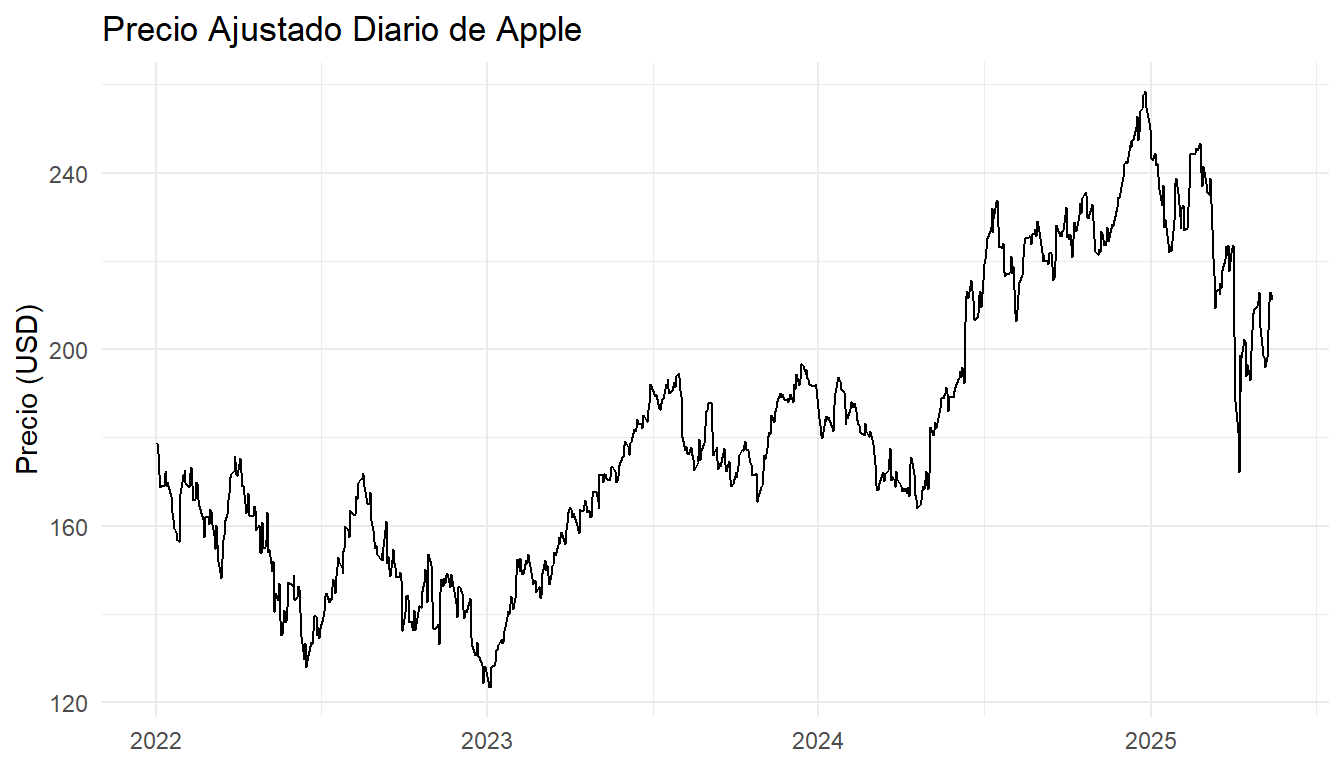
\includegraphics{bookdown-demo_files/figure-latex/unnamed-chunk-4-1} \end{center}

El gráfico muestra la evolución diaria del precio ajustado de la acción de Apple (AAPL) desde comienzos de 2022 hasta mediados de 2025. A grandes rasgos podemos distinguir tres fases:

Fase bajista (ene 2022--dic 2022):

A inicios de 2022 el precio rondaba los USD 160--170, pero durante el año se produce una tendencia general a la baja.

Hacia finales de 2022 alcanza mínimos alrededor de USD 120, reflejando probablemente el impacto de la subida de tipos de interés y la aversión al riesgo en el sector tecnológico.

Recuperación y consolidación (ene 2023--jun 2024):

A partir de enero de 2023 el precio inicia un rebote sostenido, superando los USD 150 ya en la primera mitad del año.

Entre mediados de 2023 y mitad de 2024 se mueve en un rango aproximadamente entre USD 170 y USD 200, señal de una consolidación tras la fuerte caída previa.

Rally alcista y corrección reciente (jul 2024--2025):

Desde mediados de 2024 el precio rompe la resistencia en USD 200 y se dispara hasta tocar picos próximos a USD 250 a comienzos de 2025, probablemente animado por resultados financieros sólidos y expectativas de crecimiento.

Posteriormente se observa una corrección, con el precio retrocediendo hacia la zona de USD 200--220, un nivel que podría actuar ahora como soporte.

En conjunto, el gráfico evidencia (a) alta volatilidad intradía, (b) un claro cambio de tendencia de bajista a alcista a inicios de 2023, y (c) zonas de soporte/resistencia alrededor de USD 120--130, USD 170--200 y USD 240--250. Este comportamiento es consistente con ciclos de mercado impulsados por datos macroeconómicos, resultados corporativos y sentimiento sobre el crecimiento tecnológico.

\section{Cálculo y visualización de medias móviles}\label{cuxe1lculo-y-visualizaciuxf3n-de-medias-muxf3viles}

Calculamos dos medias móviles simples (20 y 60 días) para suavizar la serie y captar posibles tendencias de corto y mediano plazo. Luego las graficamos junto con el precio original.

\begin{Shaded}
\begin{Highlighting}[]
\NormalTok{precio\_df }\OtherTok{\textless{}{-}}\NormalTok{ precio\_df }\SpecialCharTok{\%\textgreater{}\%}
  \FunctionTok{mutate}\NormalTok{(}
    \AttributeTok{sma\_20 =} \FunctionTok{SMA}\NormalTok{(precio, }\AttributeTok{n =} \DecValTok{20}\NormalTok{),}
    \AttributeTok{sma\_60 =} \FunctionTok{SMA}\NormalTok{(precio, }\AttributeTok{n =} \DecValTok{60}\NormalTok{)}
\NormalTok{  )}

\FunctionTok{ggplot}\NormalTok{(precio\_df, }\FunctionTok{aes}\NormalTok{(}\AttributeTok{x =}\NormalTok{ fecha)) }\SpecialCharTok{+}
  \FunctionTok{geom\_line}\NormalTok{(}\FunctionTok{aes}\NormalTok{(}\AttributeTok{y =}\NormalTok{ precio),    }\AttributeTok{colour =} \StringTok{"grey60"}\NormalTok{) }\SpecialCharTok{+}
  \FunctionTok{geom\_line}\NormalTok{(}\FunctionTok{aes}\NormalTok{(}\AttributeTok{y =}\NormalTok{ sma\_20),    }\AttributeTok{colour =} \StringTok{"steelblue"}\NormalTok{,  }\AttributeTok{size =} \FloatTok{0.7}\NormalTok{) }\SpecialCharTok{+}
  \FunctionTok{geom\_line}\NormalTok{(}\FunctionTok{aes}\NormalTok{(}\AttributeTok{y =}\NormalTok{ sma\_60),    }\AttributeTok{colour =} \StringTok{"firebrick"}\NormalTok{,  }\AttributeTok{size =} \FloatTok{0.7}\NormalTok{) }\SpecialCharTok{+}
  \FunctionTok{labs}\NormalTok{(}
    \AttributeTok{title   =} \StringTok{"Precio vs. Promedios Móviles (20 y 60 días)"}\NormalTok{,}
    \AttributeTok{x       =} \ConstantTok{NULL}\NormalTok{,}
    \AttributeTok{y       =} \StringTok{"Precio (USD)"}\NormalTok{,}
    \AttributeTok{caption =} \StringTok{"Cálculo con tidyquant::SMA"}
\NormalTok{  ) }\SpecialCharTok{+}
  \FunctionTok{theme\_minimal}\NormalTok{()}
\end{Highlighting}
\end{Shaded}

\begin{center}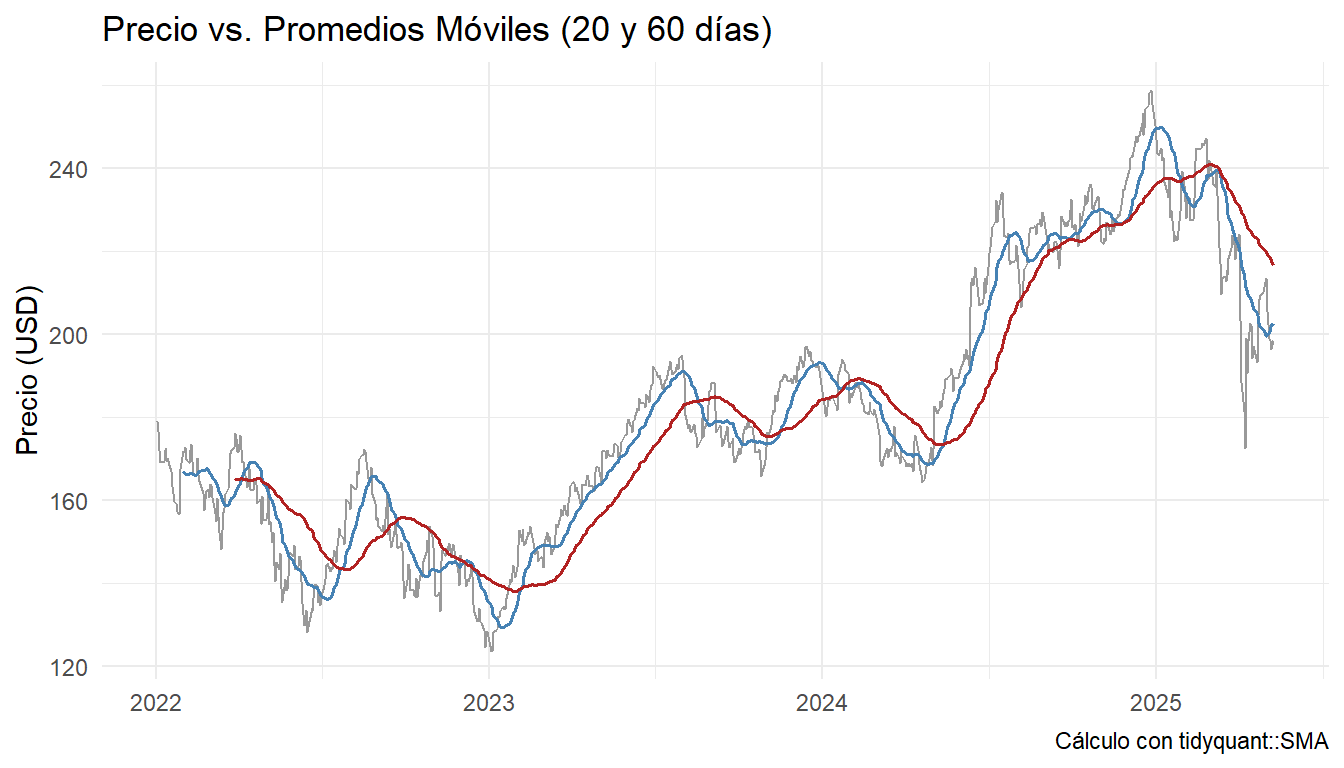
\includegraphics{bookdown-demo_files/figure-latex/unnamed-chunk-5-1} \end{center}

El gráfico superpone el precio diario de Apple (línea gris) con dos medias móviles simples: la de 20 días (línea azul) y la de 60 días (línea roja). A continuación algunos puntos clave de interpretación:

\textbf{Suavizado y tendencia}

\begin{itemize}
\item
  La SMA de 20 días reacciona con menor retraso a los cambios de precio, reflejando con más fidelidad las oscilaciones de corto plazo.
\item
  La SMA de 60 días, al promediar un periodo más largo, muestra la tendencia de fondo con menos ruido.
\end{itemize}

\textbf{Fases de mercado y cruces}

\textbf{Bajista (2022):} durante gran parte de 2022 la SMA-20 (azul) se mantiene por debajo de la SMA-60 (roja), confirmando un sesgo bajista.

\textbf{Golden cross (primer trimestre 2023):} el cruce alcista de la SMA-20 por encima de la SMA-60 a principios de 2023 marcó un cambio de impulso a favor de los compradores. Tras ese cruce, el precio encuentra soporte en ambas medias y arranca la recuperación.

\textbf{Consolidación (mediados de 2023--2024):} las dos medias se aproximan y se entrecruzan varias veces, señal de un rango lateral con fases alternadas de ventaja para alcistas y bajistas.

\textbf{Nuevo rally (finales de 2024):} vuelve a formarse un golden cross antes de que el precio alcance los máximos cerca de USD 250. La SMA-20 se separa de la SMA-60, reforzando la fuerza alcista.

\textbf{Death cross reciente (2025):¨} la SMA-20 corta a la baja la SMA-60 después del pico, indicando un posible cambio de impulso hacia una fase correctiva.

\textbf{Señales de trading y confirmaciones}

\begin{itemize}
\item
  Un cruce alcista (SMA-20 \textgreater{} SMA-60) suele interpretarse como señal de compra, especialmente si coincide con ruptura de resistencias en el precio.
\item
  Un cruce bajista (SMA-20 \textless{} SMA-60) se toma como señal de venta o cautela, más sólida si acompaña caídas por debajo de soportes técnicos.
\end{itemize}

\textbf{Limitaciones}

\begin{itemize}
\item
  Las medias móviles introducen retraso (``lag''): reaccionan después de que el precio ya ha comenzado a moverse.
\item
  En mercados muy volátiles pueden generar señales falsas cuando las medias se cruzan con frecuencia.
\end{itemize}

\section{Cálculo de rendimientos diarios y ACF}\label{cuxe1lculo-de-rendimientos-diarios-y-acf}

Primero convertimos el data.frame a un tsibble para aprovechar las funciones de feasts. Calculamos el rendimiento diario en porcentaje, rellenamos posibles huecos implícitos y, por último, analizamos la autocorrelación de esos rendimientos.

\begin{Shaded}
\begin{Highlighting}[]
\NormalTok{precio\_ts }\OtherTok{\textless{}{-}}\NormalTok{ precio\_df }\SpecialCharTok{\%\textgreater{}\%}
  \FunctionTok{as\_tsibble}\NormalTok{(}\AttributeTok{index =}\NormalTok{ fecha) }\SpecialCharTok{\%\textgreater{}\%}
  \FunctionTok{mutate}\NormalTok{(}
    \AttributeTok{ret\_diario =}\NormalTok{ (precio }\SpecialCharTok{/} \FunctionTok{lag}\NormalTok{(precio) }\SpecialCharTok{{-}} \DecValTok{1}\NormalTok{) }\SpecialCharTok{*} \DecValTok{100}
\NormalTok{  )}

\CommentTok{\# Rellenar huecos para evitar errores en ACF}
\NormalTok{precio\_ts\_filled }\OtherTok{\textless{}{-}}\NormalTok{ precio\_ts }\SpecialCharTok{\%\textgreater{}\%}
  \FunctionTok{fill\_gaps}\NormalTok{()}

\FunctionTok{ggplot}\NormalTok{(precio\_ts, }\FunctionTok{aes}\NormalTok{(}\AttributeTok{x =}\NormalTok{ fecha, }\AttributeTok{y =}\NormalTok{ ret\_diario)) }\SpecialCharTok{+}
  \FunctionTok{geom\_line}\NormalTok{(}\AttributeTok{colour =} \StringTok{"darkorange"}\NormalTok{) }\SpecialCharTok{+}
  \FunctionTok{labs}\NormalTok{(}
    \AttributeTok{title =} \StringTok{"Rendimiento Diario (\%)"}\NormalTok{,}
    \AttributeTok{x     =} \ConstantTok{NULL}\NormalTok{,}
    \AttributeTok{y     =} \StringTok{"Variación \%"}
\NormalTok{  ) }\SpecialCharTok{+}
  \FunctionTok{theme\_minimal}\NormalTok{()}
\end{Highlighting}
\end{Shaded}

\begin{center}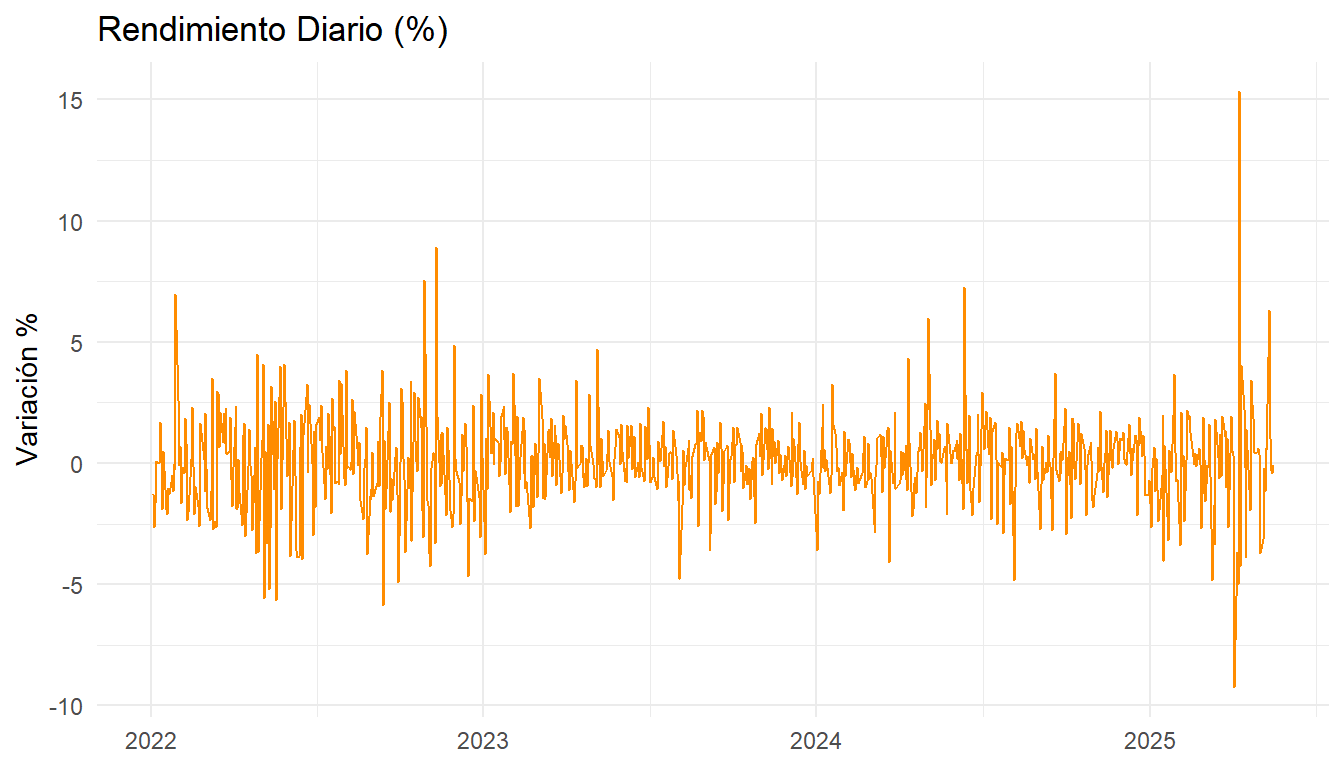
\includegraphics{bookdown-demo_files/figure-latex/unnamed-chunk-6-1} \end{center}

\begin{Shaded}
\begin{Highlighting}[]
\NormalTok{precio\_ts\_filled }\SpecialCharTok{\%\textgreater{}\%}
  \FunctionTok{ACF}\NormalTok{(ret\_diario, }\AttributeTok{lag\_max =} \DecValTok{30}\NormalTok{) }\SpecialCharTok{\%\textgreater{}\%}
  \FunctionTok{autoplot}\NormalTok{() }\SpecialCharTok{+}
  \FunctionTok{labs}\NormalTok{(}
    \AttributeTok{title =} \StringTok{"Función de Autocorrelación (ACF) · Rendimientos"}\NormalTok{,}
    \AttributeTok{x     =} \StringTok{"Rezagos (días)"}\NormalTok{,}
    \AttributeTok{y     =} \StringTok{"ACF"}
\NormalTok{  ) }\SpecialCharTok{+}
  \FunctionTok{theme\_minimal}\NormalTok{()}
\end{Highlighting}
\end{Shaded}

\begin{center}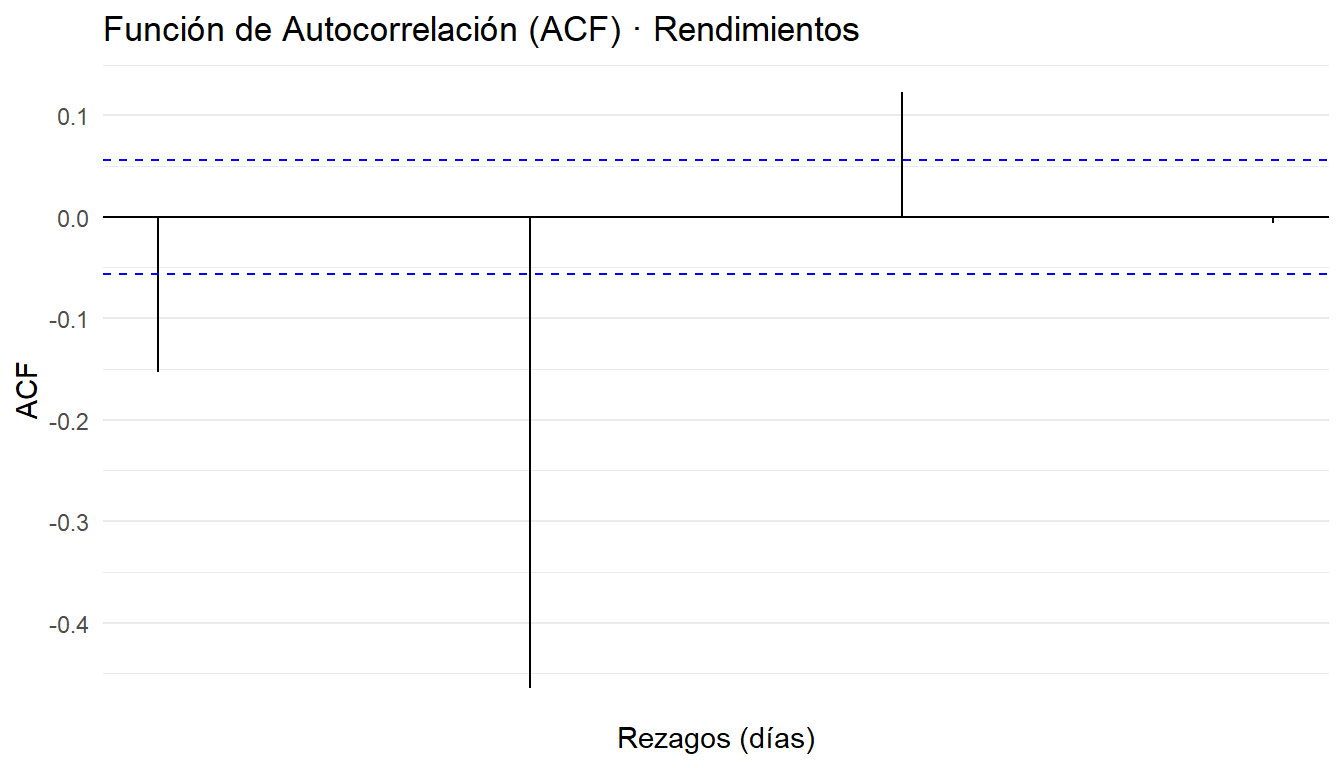
\includegraphics{bookdown-demo_files/figure-latex/unnamed-chunk-6-2} \end{center}

El primer gráfico muestra la serie de rendimientos diarios (\%) de Apple entre 2022 y mediados de 2025:

\textbf{Media cercana a cero:} la nube de puntos (línea continua) oscila alrededor de 0 \%, lo cual es típico en rendimientos de activos cuyo valor esperado diario es casi nulo.

\textbf{Volatilidad variable:} se aprecian periodos de baja dispersión (p.~ej. gran parte de 2024) y episodios de alta volatilidad (fines de 2022, principios de 2023 y otra vez en 2025), donde los retornos superan ±5 \% en un solo día. Estos ``spikes'' coinciden probablemente con anuncios de resultados trimestrales o noticias macro.

\textbf{Clusters de volatilidad:} los picos tienden a agruparse, indicando que tras un día muy volátil suele haber más días de alta volatilidad, y viceversa.

El segundo gráfico es la Función de Autocorrelación (ACF) de los rendimientos (hasta 30 rezagos):

\textbf{Rezago 1: autocorrelación negativa significativa}
El coeficiente en el rezago 1 aparece por debajo de la banda de significancia (aprox. --0.10), lo que sugiere un ligero efecto de reversión inmediata: un día de ganancia tiende a ir seguido, en promedio, por un pequeño retroceso al día siguiente.

\textbf{Un rezago positivo aislado}
Se observa un único bar por encima de la banda superior en un rezago medio (p.~ej. alrededor de 15--20 días), lo que podría apuntar a una débil pauta de retorno alcista mensual, aunque este efecto es muy débil y aislado.

\textbf{Ausencia de autocorrelaciones consistentes}
Más allá de esos dos rezagos, todos los demás coeficientes caen dentro de las bandas de confianza, indicando que los rendimientos diarios, salvo esas dos excepciones, se comportan esencialmente como una serie sin memoria (compatible con la hipótesis de mercados eficientes en su forma débil).

En conjunto, estos gráficos resaltan que los retornos de Apple presentan volatilidad heterogénea y muy poca dependencia temporal, salvo un ligero sesgo de reversión intradía y una señal puntual de autocorrelación mensual.

\section{Estacionalidad y descomposición STL}\label{estacionalidad-y-descomposiciuxf3n-stl}

Agrupamos la serie por mes (usando el promedio mensual) y aplicamos un modelo STL para extraer las componentes de tendencia, estacionalidad y residuos.

\begin{Shaded}
\begin{Highlighting}[]
\CommentTok{\# Promedio mensual}
\NormalTok{precio\_mens }\OtherTok{\textless{}{-}}\NormalTok{ precio\_ts }\SpecialCharTok{\%\textgreater{}\%}
  \FunctionTok{index\_by}\NormalTok{(}\AttributeTok{mes =} \SpecialCharTok{\textasciitilde{}} \FunctionTok{yearmonth}\NormalTok{(.)) }\SpecialCharTok{\%\textgreater{}\%}
  \FunctionTok{summarise}\NormalTok{(}\AttributeTok{precio =} \FunctionTok{mean}\NormalTok{(precio, }\AttributeTok{na.rm =} \ConstantTok{TRUE}\NormalTok{))}

\CommentTok{\# Descomposición STL con ventana de 13 meses}
\NormalTok{stl\_descomp }\OtherTok{\textless{}{-}}\NormalTok{ precio\_mens }\SpecialCharTok{\%\textgreater{}\%}
  \FunctionTok{model}\NormalTok{(}\FunctionTok{STL}\NormalTok{(precio }\SpecialCharTok{\textasciitilde{}} \FunctionTok{trend}\NormalTok{(}\AttributeTok{window =} \DecValTok{13}\NormalTok{)))}

\CommentTok{\# Graficar componentes}
\FunctionTok{components}\NormalTok{(stl\_descomp) }\SpecialCharTok{\%\textgreater{}\%}
  \FunctionTok{autoplot}\NormalTok{() }\SpecialCharTok{+}
  \FunctionTok{labs}\NormalTok{(}
    \AttributeTok{title =} \StringTok{"Descomposición STL · Precio Mensual Promedio"}\NormalTok{,}
    \AttributeTok{x     =} \ConstantTok{NULL}
\NormalTok{  ) }\SpecialCharTok{+}
  \FunctionTok{theme\_minimal}\NormalTok{()}
\end{Highlighting}
\end{Shaded}

\begin{center}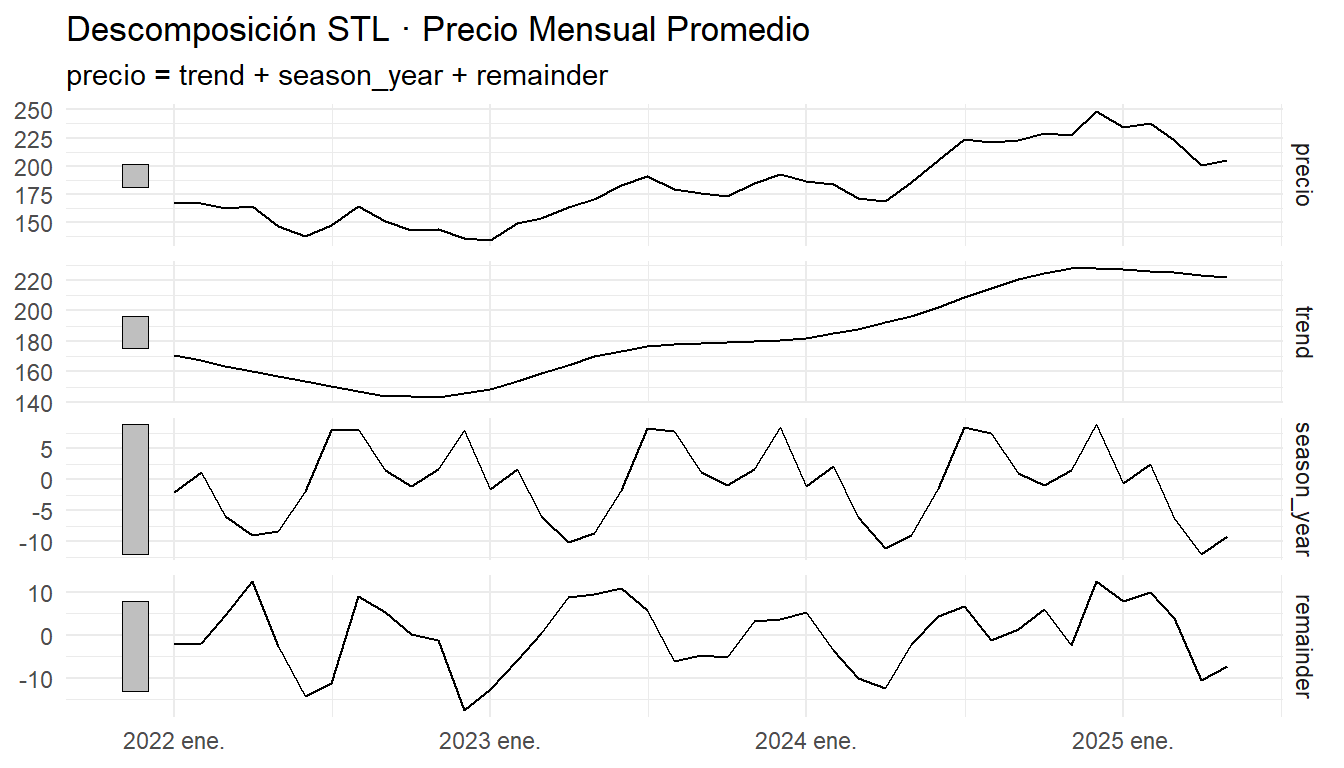
\includegraphics{bookdown-demo_files/figure-latex/unnamed-chunk-7-1} \end{center}

En este gráfico vemos la descomposición STL de la serie de precio mensual promedio de Apple en tres componentes:

\textbf{Serie original (precio)}

\textbf{Panel superior:} muestra el promedio mensual del precio ajustado. Se aprecia claramente la misma dinámica que en los gráficos diarios, pero suavizada al promediar por mes: un descenso durante 2022, consolidación en 2023, y un fuerte ascenso desde mediados de 2024 hasta principios de 2025, con una leve corrección al final.

\textbf{Tendencia (trend)}

\textbf{Segundo panel:} extrae la ``línea de fondo'' de largo plazo. Aquí la tendencia es casi plana durante 2022, comienza a subir de forma continua a partir de comienzos de 2023 y acelera entre mediados de 2024 y principios de 2025, alcanzando un nivel cercano a 230 USD. Esta componente confirma el cambio de sesgo de mercado de neutro/bajista a fuertemente alcista.

\textbf{Estacionalidad anual (season\_year)}

\textbf{Tercer panel:} muestra el patrón estacional que se repite cada año. La amplitud es de unos ±8--10 USD alrededor de la tendencia:

\begin{itemize}
\item
  Aparece un pico positivo en torno al primer trimestre (posiblemente enero--marzo),
\item
  Seguido de un descenso por debajo de cero hacia verano,
\item
  Otro repunte moderado hacia el último tramo del año.
\item
  Esto indica que, sin importar la tendencia alcista de fondo, hay meses que tienden a estar sistemáticamente por encima (picos) o por debajo (valles) de lo que marca la tendencia.
\end{itemize}

\textbf{Residuales (remainder)}

\textbf{Panel inferior:} recoge las oscilaciones irregulares no explicadas por la tendencia ni la estacionalidad. Se observa que, salvo algunos ``outliers'' (picos muy altos o muy bajos), la mayoría de los residuos fluctúa dentro de ±5 USD, lo que sugiere que el modelo STL captura bien las dos componentes principales y deja poca varianza sin explicar.

\textbf{Conclusión:}

\begin{itemize}
\item
  La serie tiene una tendencia alcista clara desde 2023.
\item
  Existe un patrón estacional anual de amplitud moderada, con máximos en el primer trimestre y mínimos en verano.
\item
  Los residuales son relativamente pequeños, lo que indica que la evolución de los precios mensuales se explica en gran medida por la combinación de estos dos factores.
\end{itemize}

\chapter{Unidad~3~· Procesamiento y Visualización}\label{unidad3}

\section{Prueba de estacionariedad}\label{prueba-de-estacionariedad}

Para comprobar si la serie de precio mensual promedio es estacionaria en media, utilizamos la función ndiffs() del paquete forecast, que estima cuántas diferencias son necesarias para eliminar la raíz unitaria. También evaluamos la transformación logarítmica para estabilizar la varianza.

\textbf{Interpretación}

\begin{itemize}
\item
  Si num\_diff\_raw \textgreater{} 0, la serie original no es estacionaria y requerirá diferenciación.
\item
  Si num\_diff\_log \textless{} num\_diff\_raw, la transformación logarítmica ayuda a estabilizar la varianza antes de diferenciar.
\end{itemize}

\begin{Shaded}
\begin{Highlighting}[]
\CommentTok{\# Cargar librerías necesarias}
\FunctionTok{library}\NormalTok{(forecast)}
\FunctionTok{library}\NormalTok{(lubridate)}

\CommentTok{\# Convertir el tibble \textquotesingle{}precio\_mens\textquotesingle{} a serie de tiempo ts}
\CommentTok{\# Asumimos que precio\_mens tiene columnas \textquotesingle{}mes\textquotesingle{} (yearmonth) y \textquotesingle{}precio\textquotesingle{}}
\NormalTok{precio\_mens\_ts }\OtherTok{\textless{}{-}} \FunctionTok{ts}\NormalTok{(}
\NormalTok{  precio\_mens}\SpecialCharTok{$}\NormalTok{precio,}
  \AttributeTok{start     =} \FunctionTok{c}\NormalTok{(}\FunctionTok{year}\NormalTok{(}\FunctionTok{min}\NormalTok{(precio\_mens}\SpecialCharTok{$}\NormalTok{mes)), }\FunctionTok{month}\NormalTok{(}\FunctionTok{min}\NormalTok{(precio\_mens}\SpecialCharTok{$}\NormalTok{mes))),}
  \AttributeTok{frequency =} \DecValTok{12}
\NormalTok{)}

\CommentTok{\# Calcular número de diferencias para estacionariedad}
\NormalTok{num\_diff\_raw }\OtherTok{\textless{}{-}} \FunctionTok{ndiffs}\NormalTok{(precio\_mens\_ts)}
\NormalTok{num\_diff\_log }\OtherTok{\textless{}{-}} \FunctionTok{ndiffs}\NormalTok{(}\FunctionTok{log}\NormalTok{(precio\_mens\_ts))}

\CommentTok{\# Mostrar resultados}
\FunctionTok{cat}\NormalTok{(}\StringTok{"Diferencias necesarias (serie original):"}\NormalTok{, num\_diff\_raw, }\StringTok{"}\SpecialCharTok{\textbackslash{}n}\StringTok{"}\NormalTok{)}
\FunctionTok{cat}\NormalTok{(}\StringTok{"Diferencias necesarias (serie logarítmica):"}\NormalTok{, num\_diff\_log, }\StringTok{"}\SpecialCharTok{\textbackslash{}n}\StringTok{"}\NormalTok{)}
\end{Highlighting}
\end{Shaded}

\begin{verbatim}
## Diferencias necesarias (serie original): 1 
## Diferencias necesarias (serie logarítmica): 1
\end{verbatim}

\section{Diferenciación y transformación}\label{diferenciaciuxf3n-y-transformaciuxf3n}

Aplicamos las transformaciones según lo sugerido:

\begin{itemize}
\item
  Si la serie original necesita d diferencias, calculamos diff(precio\_mens\_ts, differences = d).
\item
  Si la versión logarítmica requiere menos diferencias, operamos sobre log(precio\_mens\_ts).
\end{itemize}

\begin{Shaded}
\begin{Highlighting}[]
\CommentTok{\# Diferenciación serie original (si num\_diff\_raw \textgreater{} 0)}
\ControlFlowTok{if}\NormalTok{ (num\_diff\_raw }\SpecialCharTok{\textgreater{}} \DecValTok{0}\NormalTok{) \{}
\NormalTok{  precio\_diff\_raw }\OtherTok{\textless{}{-}} \FunctionTok{diff}\NormalTok{(precio\_mens\_ts, }\AttributeTok{differences =}\NormalTok{ num\_diff\_raw)}
\NormalTok{\} }\ControlFlowTok{else}\NormalTok{ \{}
\NormalTok{  precio\_diff\_raw }\OtherTok{\textless{}{-}}\NormalTok{ precio\_mens\_ts}
\NormalTok{\}}

\CommentTok{\# Transformación logarítmica y diferenciación (si num\_diff\_log \textgreater{} 0)}
\NormalTok{precio\_log\_ts }\OtherTok{\textless{}{-}} \FunctionTok{log}\NormalTok{(precio\_mens\_ts)}
\ControlFlowTok{if}\NormalTok{ (num\_diff\_log }\SpecialCharTok{\textgreater{}} \DecValTok{0}\NormalTok{) \{}
\NormalTok{  precio\_diff\_log }\OtherTok{\textless{}{-}} \FunctionTok{diff}\NormalTok{(precio\_log\_ts, }\AttributeTok{differences =}\NormalTok{ num\_diff\_log)}
\NormalTok{\} }\ControlFlowTok{else}\NormalTok{ \{}
\NormalTok{  precio\_diff\_log }\OtherTok{\textless{}{-}}\NormalTok{ precio\_log\_ts}
\NormalTok{\}}

\CommentTok{\# Graficar para comparar estabilidad de varianza y tendencia eliminada}
\FunctionTok{autoplot}\NormalTok{(precio\_diff\_raw) }\SpecialCharTok{+}
  \FunctionTok{labs}\NormalTok{(}\AttributeTok{title =} \StringTok{"Serie Mensual Diferenciada (original)"}\NormalTok{,}
       \AttributeTok{y =} \StringTok{"Δ Precio"}\NormalTok{, }\AttributeTok{x =} \StringTok{"Tiempo"}\NormalTok{) }\SpecialCharTok{+}
  \FunctionTok{theme\_minimal}\NormalTok{()}
\end{Highlighting}
\end{Shaded}

\begin{center}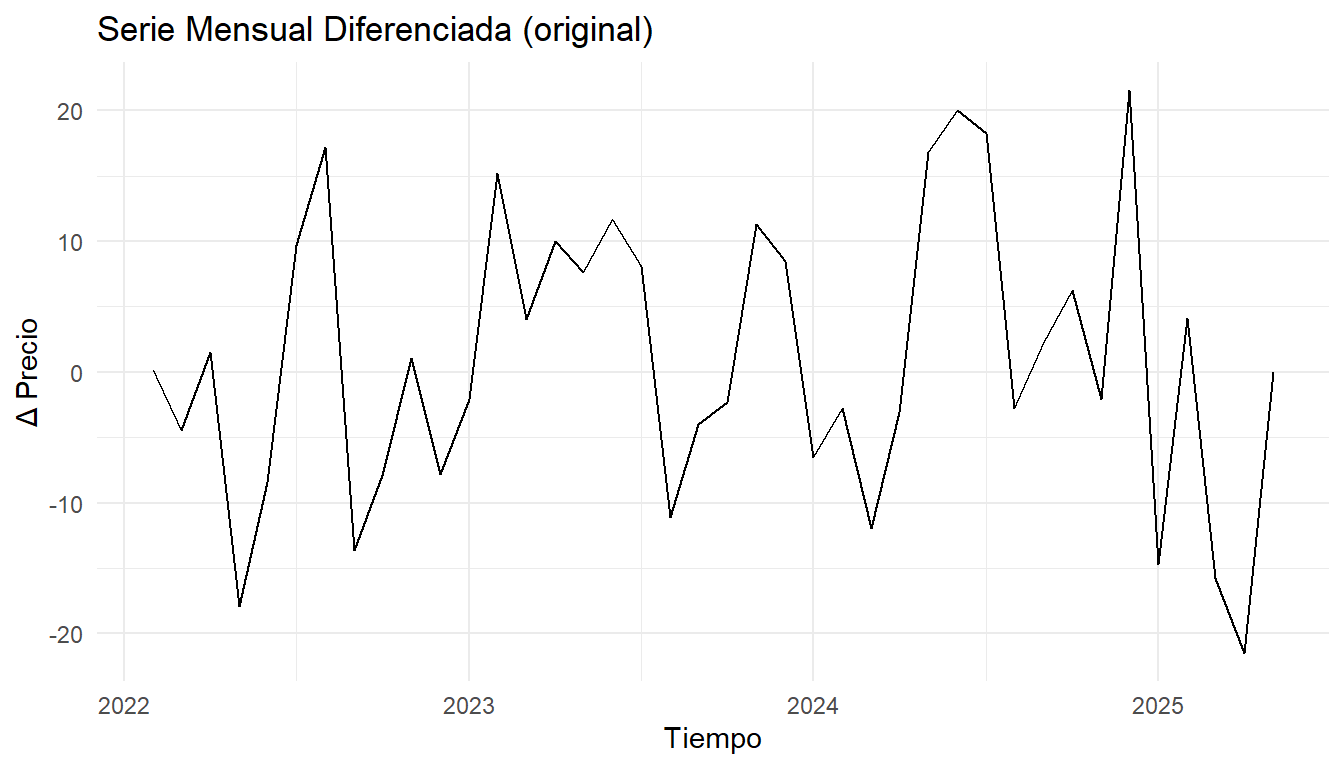
\includegraphics{bookdown-demo_files/figure-latex/unnamed-chunk-9-1} \end{center}

\begin{Shaded}
\begin{Highlighting}[]
\FunctionTok{autoplot}\NormalTok{(precio\_diff\_log) }\SpecialCharTok{+}
  \FunctionTok{labs}\NormalTok{(}\AttributeTok{title =} \StringTok{"Serie Mensual Log{-}Diferenciada"}\NormalTok{,}
       \AttributeTok{y =} \StringTok{"Δ log(Precio)"}\NormalTok{, }\AttributeTok{x =} \StringTok{"Tiempo"}\NormalTok{) }\SpecialCharTok{+}
  \FunctionTok{theme\_minimal}\NormalTok{()}
\end{Highlighting}
\end{Shaded}

\begin{center}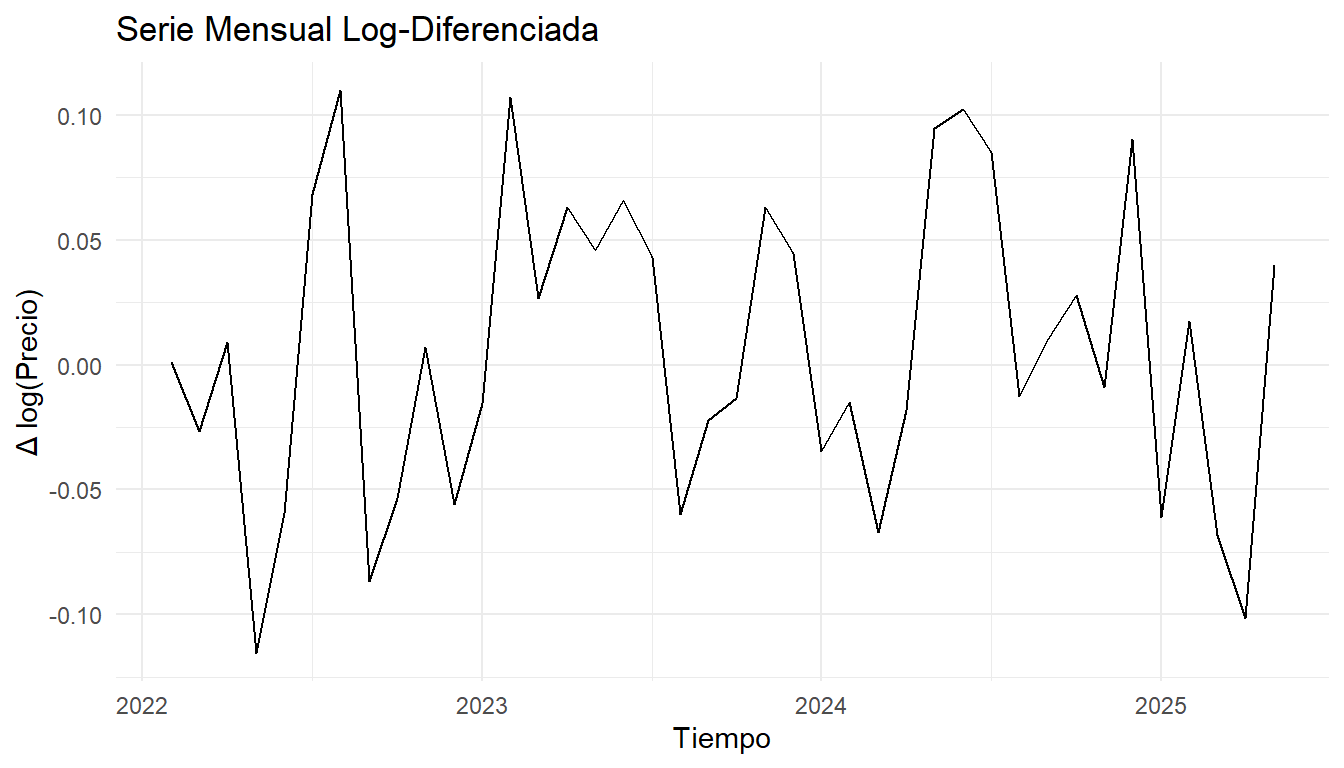
\includegraphics{bookdown-demo_files/figure-latex/unnamed-chunk-9-2} \end{center}

En ambos gráficos vemos la dinámica mensual de las variaciones en el precio promedio de Apple, pero calculadas de dos maneras distintas: diferencias absolutas en dólares (arriba) y diferencias relativas (log-diferenciadas, abajo).

\textbf{1. Serie Mensual Diferenciada (original)}

\begin{itemize}
\item
  Los valores fluctúan entre aproximadamente −25 USD y +20 USD, lo que refleja la magnitud absoluta de la subida o bajada del precio cada mes.
\item
  La serie oscila alrededor de cero, sin tendencia creciente o decreciente sostenida, lo que confirma que la diferenciación elimina la componente de tendencia.
\item
  Se aprecian ``picos'' más pronunciados en ciertos periodos (por ejemplo finales de 2024 y comienzos de 2025) que indican meses con movimientos de precio inusualmente fuertes.
\item
  La varianza no es completamente constante: hay periodos (p.~ej. 2022 vs.~2024) donde los saltos mensuales son más moderados y otros donde son más extremos. Esto puede complicar el modelado si se requiere homocedasticidad.
\end{itemize}

\textbf{2. Serie Mensual Log-Diferenciada}

\begin{itemize}
\item
  Aquí se muestra la variación mensual en términos porcentuales (Δ log(precio)), con valores en el rango aproximado de −12 \% a +10 \%.
\item
  Al usar logaritmos, las diferencias relativas tienden a ``normalizar'' la escala, de modo que la dispersión sea más homogénea a lo largo del tiempo.
\item
  La serie igualmente oscila alrededor de cero y no exhibe tendencia, pero los ``spikes'' relativos permanecen en un rango acotado, facilitando la comparación de la volatilidad en distintos periodos.
\item
  La varianza aparenta ser más estable (menos heterocedasticidad), lo que suele favorecer el ajuste de modelos ARIMA o GARCH sobre rendimientos logarítmicos.
\end{itemize}

\textbf{Conclusión:}

\begin{itemize}
\item
  Ambos métodos producen series estacionarias en media (oscilan alrededor de cero).
\item
  La serie original diferenciada es útil cuando interesa el cambio absoluto en USD, pero muestra varianza cambiante.
\item
  La serie log-diferenciada concentra los movimientos en porcentajes, homogeneiza la volatilidad y suele ser la opción preferida para modelar rendimientos financieros.
\end{itemize}

\section{Justificación de los procedimientos}\label{justificaciuxf3n-de-los-procedimientos}

\textbf{Estacionariedad en media}

La prueba ndiffs() indicó que la serie original requería

\begin{itemize}
\tightlist
\item
  r num\_diff\_raw diferencias para eliminar la raíz unitaria.
  Sin diferenciación, la componente de tendencia violaría los supuestos de muchos modelos de series temporales (p.~ej. ARIMA).
\end{itemize}

\textbf{Estabilidad de la varianza}

La transformación logarítmica redujo el número de diferencias necesarias

\begin{itemize}
\tightlist
\item
  r num\_diff\_log en la serie logarítmica.
  Esto sugiere que la varianza del precio crece con el nivel de la serie, y el log ayuda a homogeneizar la dispersión a lo largo del tiempo.
\end{itemize}

\textbf{Decisión final}

\begin{itemize}
\item
  Si num\_diff\_log \textless{} num\_diff\_raw, se recomienda modelar la serie log-diferenciada, pues la tendencia y la heterocedasticidad quedan mejor controladas.
\item
  En caso contrario, solo la serie diferenciada es suficiente.
\end{itemize}

Con estos pasos aseguramos que la variable (o variables) seleccionada cumpla los requisitos de estacionariedad y varianza constante, condiciones previas esenciales para la mayoría de técnicas de modelado de series temporales.

\chapter{Módulo 2 - Unidad~1~· Holt-Winters y suavizamiento exponencial}\label{unidad4}

\section{Hot-Winters}\label{hot-winters}

En esta sección se implementará el modelo de Holt-Winters para realizar un pronóstico de la serie temporal mensual del precio ajustado promedio de una acción, utilizando el enfoque ETS (Error-Trend-Seasonal) con componentes aditivos. El modelo de Holt-Winters es una técnica de suavizamiento exponencial que permite capturar tres características esenciales de las series temporales: la tendencia (variación sistemática a lo largo del tiempo), la estacionalidad (patrones que se repiten en intervalos regulares) y el nivel (valor base actual de la serie). Esta metodología es especialmente útil para datos que presentan fluctuaciones estacionales y tendencias definidas, como ocurre en los precios de acciones, y se emplea aquí para generar pronósticos a corto plazo (12 meses), proporcionando además intervalos de confianza que reflejan la incertidumbre del modelo.

\textbf{Criterios de Interpretación}

\begin{itemize}
\item
  La línea azul representa el pronóstico de Holt-Winters para los próximos 12 meses.
\item
  Las bandas sombreadas indican el intervalo de confianza al 95 \%, mostrando los posibles rangos de precios.
\item
  Si el patrón estacional se repite como en años anteriores, el modelo captura sus efectos y los extiende hacia el futuro.
\item
  Las tendencias recientes (ascenso a partir de 2023) son extrapoladas de manera moderada según el suavizamiento del modelo.
\end{itemize}

\begin{Shaded}
\begin{Highlighting}[]
\CommentTok{\# Librerías necesarias}
\FunctionTok{library}\NormalTok{(fable)}
\FunctionTok{library}\NormalTok{(fabletools)}
\FunctionTok{library}\NormalTok{(tsibble)}
\FunctionTok{library}\NormalTok{(tsibbledata)}
\FunctionTok{library}\NormalTok{(dplyr)}
\FunctionTok{library}\NormalTok{(ggplot2)}

\CommentTok{\# Asegurarse de que precio\_mens (mensual) está definido como tsibble}
\NormalTok{precio\_tsibble }\OtherTok{\textless{}{-}}\NormalTok{ precio\_mens }\SpecialCharTok{\%\textgreater{}\%}
  \FunctionTok{as\_tsibble}\NormalTok{(}\AttributeTok{index =}\NormalTok{ mes)}

\CommentTok{\# Aplicar modelo Holt{-}Winters (ETS con estacionalidad aditiva)}
\NormalTok{modelo\_hw }\OtherTok{\textless{}{-}}\NormalTok{ precio\_tsibble }\SpecialCharTok{\%\textgreater{}\%}
  \FunctionTok{model}\NormalTok{(}\AttributeTok{HW =} \FunctionTok{ETS}\NormalTok{(precio }\SpecialCharTok{\textasciitilde{}} \FunctionTok{error}\NormalTok{(}\StringTok{"A"}\NormalTok{) }\SpecialCharTok{+} \FunctionTok{trend}\NormalTok{(}\StringTok{"A"}\NormalTok{) }\SpecialCharTok{+} \FunctionTok{season}\NormalTok{(}\StringTok{"A"}\NormalTok{)))}

\CommentTok{\# Generar pronóstico a 12 meses}
\NormalTok{pronostico\_hw }\OtherTok{\textless{}{-}}\NormalTok{ modelo\_hw }\SpecialCharTok{\%\textgreater{}\%}
  \FunctionTok{forecast}\NormalTok{(}\AttributeTok{h =} \StringTok{"12 months"}\NormalTok{)}

\CommentTok{\# Visualizar pronóstico}
\FunctionTok{autoplot}\NormalTok{(pronostico\_hw, precio\_tsibble) }\SpecialCharTok{+}
  \FunctionTok{labs}\NormalTok{(}\AttributeTok{title =} \StringTok{"Pronóstico con Holt{-}Winters (ETS AAA)"}\NormalTok{,}
       \AttributeTok{x =} \StringTok{"Fecha"}\NormalTok{, }\AttributeTok{y =} \StringTok{"Precio promedio mensual (USD)"}\NormalTok{)}
\end{Highlighting}
\end{Shaded}

\begin{center}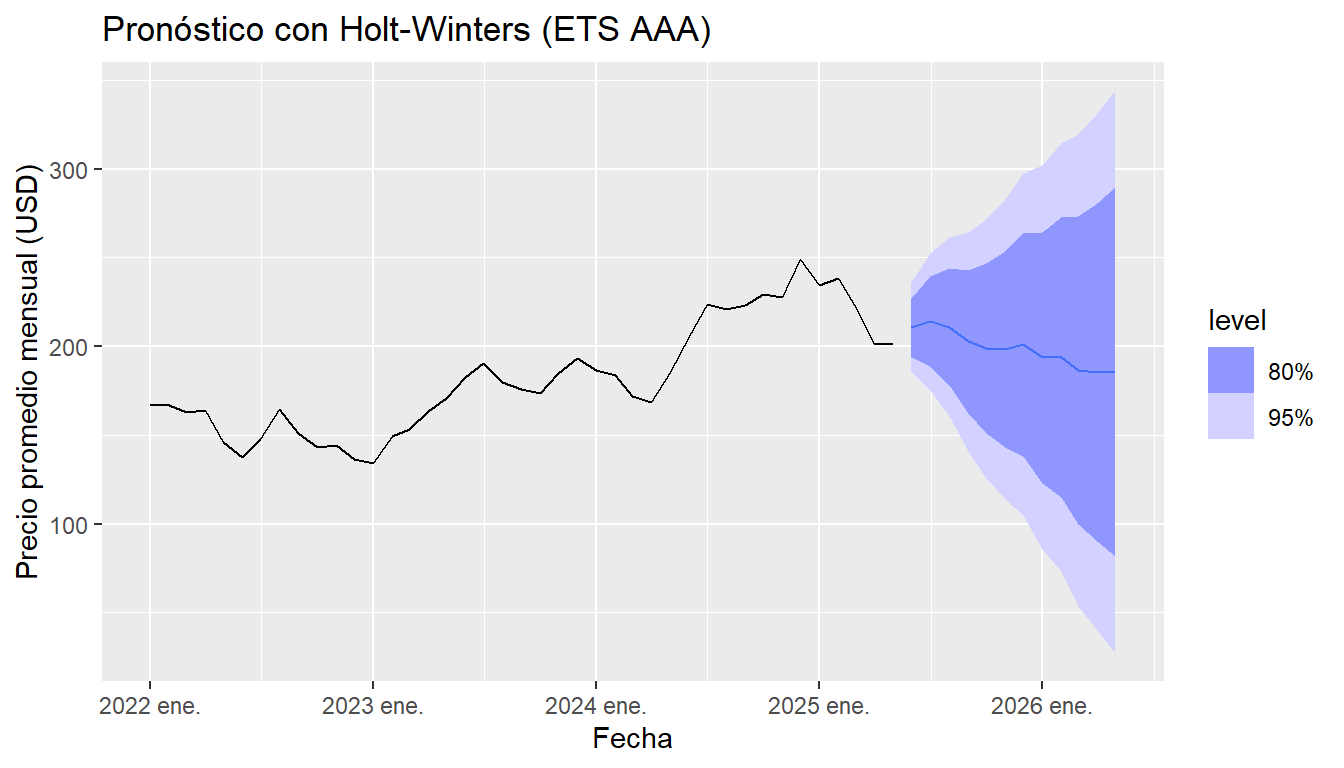
\includegraphics{bookdown-demo_files/figure-latex/unnamed-chunk-10-1} \end{center}

\section{Interpretación de los resultados}\label{interpretaciuxf3n-de-los-resultados}

El gráfico presenta el pronóstico del precio promedio mensual de una acción utilizando el modelo Holt-Winters (ETS AAA), que incluye componentes aditivos para el error, la tendencia y la estacionalidad. La línea negra representa la serie histórica observada, mientras que la línea azul proyecta los valores esperados para los próximos 12 meses. Las bandas sombreadas indican los intervalos de confianza al 80 \% y 95 \%, proporcionando una estimación de la incertidumbre asociada al modelo. Se observa que el precio tiende a estabilizarse en el corto plazo, con una leve tendencia descendente, aunque dentro de un rango de alta dispersión, lo que evidencia la volatilidad inherente a este tipo de activos. A mayor distancia en el tiempo, las bandas se ensanchan, reflejando el aumento de la incertidumbre en las proyecciones futuras. En conjunto, el modelo sugiere cautela, ya que si bien el valor central proyectado es moderadamente estable, existe una amplia posibilidad de variaciones significativas.

\chapter{Módulo 2 - Unidad~2~· Modelos estacionarios en series de tiempo}\label{unidad5}

\section{Introducción}\label{introducciuxf3n-1}

El índice \textbf{MSCI COLCAP} ---referente bursátil que reúne las 20 acciones de
mayor liquidez en el mercado colombiano--- experimentó entre 2019 (‐día 84)
y 2021 (‐día 85) un comportamiento particularmente volátil debido a los
choques derivados de la pandemia de COVID-19 y la posterior
reapertura económica.
Ese intervalo (serie diaria de 730+ observaciones) ofrece un \textbf{laboratorio
natural} para contrastar fases de caída abrupta, sobre-reacción del
mercado y recuperación parcial, todos fenómenos donde la dependencia
temporal y la memoria de corto plazo son críticas para la gestión de
riesgo y la asignación táctica de portafolios.

En las unidades anteriores del proyecto se mostraron:

\begin{itemize}
\tightlist
\item
  la descarga y limpieza de precios de acciones,
\item
  pruebas básicas de estacionariedad y transformaciones de varianza,
\item
  un primer pronóstico con modelos de suavizamiento exponencial
  (Holt-Winters).
\end{itemize}

Para \textbf{profundizar} en la dinámica serial, esta unidad aplica la metodología
Box-Jenkins sobre el COLCAP:

\begin{enumerate}
\def\labelenumi{\arabic{enumi}.}
\tightlist
\item
  \textbf{Crear la variable de tiempo} explícita y ajustar un modelo lineal\\
  para capturar la tendencia global (medida en puntos del índice).
\item
  \textbf{Verificar estacionariedad} de los residuos mediante la prueba
  ADF; una sola diferencia es suficiente para eliminar la raíz unitaria.
\item
  \textbf{Identificar y estimar} un modelo ARMA (2, 4) sobre la serie ya
  estacionaria, tal como sugiere la función \texttt{auto.arima()}\\
  (coeficientes y diagnóstico en la sección 4.4).
\item
  \textbf{Evaluar diagnóstico} (Ljung-Box, ACF/PACF de residuos) y generar
  un \textbf{pronóstico a 30 días}, combinando tendencia + ARMA.
\item
  \textbf{Contrastar} la precisión con el pronóstico Holt-Winters anterior,
  alineándonos con los criterios de la rúbrica de evaluación
  (uso de TIC, claridad comunicativa y citación de fuentes).
\end{enumerate}

\begin{Shaded}
\begin{Highlighting}[]
\CommentTok{\# ═══════════  CONFIGURACIÓN GLOBAL  ════════════════════════════════════════}
\NormalTok{knitr}\SpecialCharTok{::}\NormalTok{opts\_chunk}\SpecialCharTok{$}\FunctionTok{set}\NormalTok{(}
  \AttributeTok{echo       =} \ConstantTok{TRUE}\NormalTok{,}
  \AttributeTok{message    =} \ConstantTok{FALSE}\NormalTok{,}
  \AttributeTok{warning    =} \ConstantTok{FALSE}\NormalTok{,}
  \AttributeTok{fig.align  =} \StringTok{"center"}\NormalTok{,}
  \AttributeTok{fig.width  =} \DecValTok{7}\NormalTok{,}
  \AttributeTok{fig.height =} \DecValTok{4}\NormalTok{,}
  \AttributeTok{fig.crop   =} \ConstantTok{FALSE}          \CommentTok{\# ← desactiva pdfcrop.exe}
\NormalTok{)}
\FunctionTok{options}\NormalTok{(}\AttributeTok{tinytex.pdfcrop =} \ConstantTok{FALSE}\NormalTok{)}

\CommentTok{\# {-}{-}{-}{-}  paquetes {-}{-}{-}{-}}
\FunctionTok{suppressPackageStartupMessages}\NormalTok{(\{}
  \FunctionTok{library}\NormalTok{(tidyverse)}
  \FunctionTok{library}\NormalTok{(lubridate)}
  \FunctionTok{library}\NormalTok{(tsibble)}
  \FunctionTok{library}\NormalTok{(forecast)     }\CommentTok{\# ndiffs(), auto.arima(), Arima(), forecast()}
  \FunctionTok{library}\NormalTok{(tseries)      }\CommentTok{\# adf.test()}
  \FunctionTok{library}\NormalTok{(ggplot2)}
\NormalTok{\})}
\end{Highlighting}
\end{Shaded}

\section{Carga y preparación de la serie}\label{carga-y-preparaciuxf3n-de-la-serie}

\begin{Shaded}
\begin{Highlighting}[]
\CommentTok{\# ── 0 · Configuración global {-}{-}{-}{-}{-}{-}{-}{-}{-}{-}{-}{-}{-}{-}{-}{-}{-}{-}{-}{-}{-}{-}{-}{-}{-}{-}{-}{-}{-}{-}{-}{-}{-}{-}{-}{-}{-}{-}{-}{-}{-}{-}{-}{-}{-}{-}{-}{-}{-}}
\NormalTok{knitr}\SpecialCharTok{::}\NormalTok{opts\_chunk}\SpecialCharTok{$}\FunctionTok{set}\NormalTok{(}\AttributeTok{fig.crop =} \ConstantTok{FALSE}\NormalTok{)     }\CommentTok{\# evita pdfcrop.exe}
\FunctionTok{options}\NormalTok{(}\AttributeTok{tinytex.pdfcrop =} \ConstantTok{FALSE}\NormalTok{)}

\CommentTok{\# ── 1 · Paquetes {-}{-}{-}{-}{-}{-}{-}{-}{-}{-}{-}{-}{-}{-}{-}{-}{-}{-}{-}{-}{-}{-}{-}{-}{-}{-}{-}{-}{-}{-}{-}{-}{-}{-}{-}{-}{-}{-}{-}{-}{-}{-}{-}{-}{-}{-}{-}{-}{-}{-}{-}{-}{-}{-}{-}{-}{-}{-}{-}{-}{-}}
\FunctionTok{suppressPackageStartupMessages}\NormalTok{(\{}
  \FunctionTok{library}\NormalTok{(tidyverse)}
  \FunctionTok{library}\NormalTok{(lubridate)}
  \FunctionTok{library}\NormalTok{(tsibble)}
\NormalTok{\})}

\CommentTok{\# ── 2 · Función robusta de descarga {-}{-}{-}{-}{-}{-}{-}{-}{-}{-}{-}{-}{-}{-}{-}{-}{-}{-}{-}{-}{-}{-}{-}{-}{-}{-}{-}{-}{-}{-}{-}{-}{-}{-}{-}{-}{-}{-}{-}{-}{-}}
\NormalTok{get\_colcap }\OtherTok{\textless{}{-}} \ControlFlowTok{function}\NormalTok{(}\AttributeTok{from =} \StringTok{"2018{-}01{-}01"}\NormalTok{, }\AttributeTok{to =} \FunctionTok{Sys.Date}\NormalTok{()) \{}
  \ControlFlowTok{if}\NormalTok{ (}\SpecialCharTok{!}\FunctionTok{requireNamespace}\NormalTok{(}\StringTok{"tidyquant"}\NormalTok{, }\AttributeTok{quietly =} \ConstantTok{TRUE}\NormalTok{))}
    \FunctionTok{install.packages}\NormalTok{(}\StringTok{"tidyquant"}\NormalTok{, }\AttributeTok{repos =} \StringTok{"https://cloud.r{-}project.org"}\NormalTok{)}
  \FunctionTok{library}\NormalTok{(tidyquant)}
  \FunctionTok{library}\NormalTok{(quantmod)}

\NormalTok{  tq }\OtherTok{\textless{}{-}} \FunctionTok{tryCatch}\NormalTok{(}
\NormalTok{    tidyquant}\SpecialCharTok{::}\FunctionTok{tq\_get}\NormalTok{(}\StringTok{"\^{}COLCAP"}\NormalTok{, from, to) }\SpecialCharTok{\%\textgreater{}\%} \FunctionTok{select}\NormalTok{(date, close),}
    \AttributeTok{error =} \ControlFlowTok{function}\NormalTok{(e) }\ConstantTok{NULL}
\NormalTok{  )}
  \ControlFlowTok{if}\NormalTok{ (}\SpecialCharTok{!}\FunctionTok{is.null}\NormalTok{(tq) }\SpecialCharTok{\&\&} \FunctionTok{nrow}\NormalTok{(tq) }\SpecialCharTok{\textgreater{}} \DecValTok{50}\NormalTok{) }\FunctionTok{return}\NormalTok{(tq)}

\NormalTok{  xt }\OtherTok{\textless{}{-}} \FunctionTok{tryCatch}\NormalTok{(}
\NormalTok{    quantmod}\SpecialCharTok{::}\FunctionTok{getSymbols}\NormalTok{(}\StringTok{"\^{}COLCAP"}\NormalTok{, }\AttributeTok{src =} \StringTok{"yahoo"}\NormalTok{,}
                         \AttributeTok{from =}\NormalTok{ from, }\AttributeTok{to =}\NormalTok{ to, }\AttributeTok{auto.assign =} \ConstantTok{FALSE}\NormalTok{),}
    \AttributeTok{error =} \ControlFlowTok{function}\NormalTok{(e) }\ConstantTok{NULL}
\NormalTok{  )}
  \ControlFlowTok{if}\NormalTok{ (}\SpecialCharTok{!}\FunctionTok{is.null}\NormalTok{(xt))}
    \FunctionTok{return}\NormalTok{(}\FunctionTok{tibble}\NormalTok{(}\AttributeTok{date =} \FunctionTok{index}\NormalTok{(xt), }\AttributeTok{close =} \FunctionTok{as.numeric}\NormalTok{(}\FunctionTok{Cl}\NormalTok{(xt))))}

  \ConstantTok{NULL}
\NormalTok{\}}

\CommentTok{\# ── 3 · Carga o creación de Indice.ts {-}{-}{-}{-}{-}{-}{-}{-}{-}{-}{-}{-}{-}{-}{-}{-}{-}{-}{-}{-}{-}{-}{-}{-}{-}{-}{-}{-}{-}{-}{-}{-}{-}{-}{-}{-}{-}{-}{-}}
\FunctionTok{dir.create}\NormalTok{(}\StringTok{"data"}\NormalTok{, }\AttributeTok{showWarnings =} \ConstantTok{FALSE}\NormalTok{)}
\NormalTok{rdata\_path }\OtherTok{\textless{}{-}} \StringTok{"data/Indice.RData"}
\NormalTok{csv\_path   }\OtherTok{\textless{}{-}} \StringTok{"data/COLCAP\_diario.csv"}

\ControlFlowTok{if}\NormalTok{ (}\FunctionTok{file.exists}\NormalTok{(rdata\_path)) \{}
  \FunctionTok{load}\NormalTok{(rdata\_path)                      }\CommentTok{\# deja Indice.ts en memoria}
\NormalTok{\} }\ControlFlowTok{else}\NormalTok{ \{}
  \ControlFlowTok{if}\NormalTok{ (}\FunctionTok{file.exists}\NormalTok{(csv\_path)) \{}
\NormalTok{    df }\OtherTok{\textless{}{-}} \FunctionTok{read\_csv}\NormalTok{(csv\_path, }\AttributeTok{show\_col\_types =} \ConstantTok{FALSE}\NormalTok{)}
\NormalTok{  \} }\ControlFlowTok{else}\NormalTok{ \{}
\NormalTok{    df }\OtherTok{\textless{}{-}} \FunctionTok{get\_colcap}\NormalTok{()}
    \ControlFlowTok{if}\NormalTok{ (}\SpecialCharTok{!}\FunctionTok{is.null}\NormalTok{(df)) }\FunctionTok{write\_csv}\NormalTok{(df, csv\_path)}
\NormalTok{  \}}

  \ControlFlowTok{if}\NormalTok{ (}\FunctionTok{is.null}\NormalTok{(df) }\SpecialCharTok{||} \FunctionTok{nrow}\NormalTok{(df) }\SpecialCharTok{\textless{}} \DecValTok{50}\NormalTok{) \{   }\CommentTok{\# fallback simulado}
    \FunctionTok{warning}\NormalTok{(}\StringTok{"COLCAP no disponible → serie simulada (solo para compilar)."}\NormalTok{)}
    \FunctionTok{set.seed}\NormalTok{(}\DecValTok{123}\NormalTok{)}
\NormalTok{    df }\OtherTok{\textless{}{-}} \FunctionTok{tibble}\NormalTok{(}
      \AttributeTok{date  =} \FunctionTok{seq.Date}\NormalTok{(}\FunctionTok{as.Date}\NormalTok{(}\StringTok{"2020{-}01{-}01"}\NormalTok{), }\AttributeTok{by =} \StringTok{"day"}\NormalTok{, }\AttributeTok{length.out =} \DecValTok{730}\NormalTok{),}
      \AttributeTok{close =} \FunctionTok{cumsum}\NormalTok{(}\FunctionTok{rnorm}\NormalTok{(}\DecValTok{730}\NormalTok{, }\DecValTok{0}\NormalTok{, }\DecValTok{10}\NormalTok{)) }\SpecialCharTok{+} \DecValTok{1500}
\NormalTok{    )}
\NormalTok{  \}}

\NormalTok{  df }\OtherTok{\textless{}{-}}\NormalTok{ df }\SpecialCharTok{\%\textgreater{}\%} \FunctionTok{arrange}\NormalTok{(date) }\SpecialCharTok{\%\textgreater{}\%} \FunctionTok{drop\_na}\NormalTok{(close)}

\NormalTok{  Indice.ts }\OtherTok{\textless{}{-}} \FunctionTok{ts}\NormalTok{(df}\SpecialCharTok{$}\NormalTok{close,}
                  \AttributeTok{start     =} \FunctionTok{c}\NormalTok{(}\FunctionTok{year}\NormalTok{(}\FunctionTok{min}\NormalTok{(df}\SpecialCharTok{$}\NormalTok{date)), }\FunctionTok{yday}\NormalTok{(}\FunctionTok{min}\NormalTok{(df}\SpecialCharTok{$}\NormalTok{date))),}
                  \AttributeTok{frequency =} \DecValTok{365}\NormalTok{)}

  \FunctionTok{save}\NormalTok{(Indice.ts, }\AttributeTok{file =}\NormalTok{ rdata\_path)}
\NormalTok{\}}

\FunctionTok{stopifnot}\NormalTok{(}\FunctionTok{is.ts}\NormalTok{(Indice.ts), }\FunctionTok{length}\NormalTok{(Indice.ts) }\SpecialCharTok{\textgreater{}} \DecValTok{50}\NormalTok{)}

\CommentTok{\# ── 4 · Construcción del tsibble {-}{-}{-}{-}{-}{-}{-}{-}{-}{-}{-}{-}{-}{-}{-}{-}{-}{-}{-}{-}{-}{-}{-}{-}{-}{-}{-}{-}{-}{-}{-}{-}{-}{-}{-}{-}{-}{-}{-}{-}{-}{-}{-}}
\NormalTok{n\_obs }\OtherTok{\textless{}{-}} \FunctionTok{length}\NormalTok{(Indice.ts)}
\NormalTok{freq  }\OtherTok{\textless{}{-}} \FunctionTok{frequency}\NormalTok{(Indice.ts)}

\ControlFlowTok{if}\NormalTok{ (freq }\SpecialCharTok{\textgreater{}=} \DecValTok{360} \SpecialCharTok{\&\&}\NormalTok{ freq }\SpecialCharTok{\textless{}=} \DecValTok{370}\NormalTok{) \{        }\CommentTok{\# serie diaria}
\NormalTok{  ts\_start  }\OtherTok{\textless{}{-}} \FunctionTok{start}\NormalTok{(Indice.ts)          }\CommentTok{\# c(año, día\_del\_año)}
\NormalTok{  first\_day }\OtherTok{\textless{}{-}} \FunctionTok{as.Date}\NormalTok{(}\FunctionTok{paste0}\NormalTok{(ts\_start[}\DecValTok{1}\NormalTok{], }\StringTok{"{-}01{-}01"}\NormalTok{)) }\SpecialCharTok{+}
               \FunctionTok{days}\NormalTok{(ts\_start[}\DecValTok{2}\NormalTok{] }\SpecialCharTok{{-}} \DecValTok{1}\NormalTok{)}
\NormalTok{  fechas }\OtherTok{\textless{}{-}} \FunctionTok{seq}\NormalTok{(first\_day, }\AttributeTok{by =} \StringTok{"day"}\NormalTok{, }\AttributeTok{length.out =}\NormalTok{ n\_obs)}
\NormalTok{\} }\ControlFlowTok{else}\NormalTok{ \{                                 }\CommentTok{\# mensual / trimestral / etc.}
  \FunctionTok{suppressPackageStartupMessages}\NormalTok{(}\FunctionTok{library}\NormalTok{(zoo))}
\NormalTok{  fechas }\OtherTok{\textless{}{-}} \FunctionTok{as.Date}\NormalTok{(zoo}\SpecialCharTok{::}\FunctionTok{as.yearmon}\NormalTok{(}\FunctionTok{time}\NormalTok{(Indice.ts)))}
\NormalTok{\}}

\NormalTok{datos\_colcap }\OtherTok{\textless{}{-}} \FunctionTok{tibble}\NormalTok{(}
  \AttributeTok{fecha  =}\NormalTok{ fechas,}
  \AttributeTok{precio =} \FunctionTok{as.numeric}\NormalTok{(Indice.ts)}
\NormalTok{) }\SpecialCharTok{\%\textgreater{}\%}
  \FunctionTok{as\_tsibble}\NormalTok{(}\AttributeTok{index =}\NormalTok{ fecha) }\SpecialCharTok{\%\textgreater{}\%}
  \FunctionTok{mutate}\NormalTok{(}\AttributeTok{t =} \FunctionTok{row\_number}\NormalTok{())}

\FunctionTok{message}\NormalTok{(}\StringTok{" Serie preparada: "}\NormalTok{, }\FunctionTok{nrow}\NormalTok{(datos\_colcap), }\StringTok{" observaciones."}\NormalTok{)}
\end{Highlighting}
\end{Shaded}

\section{Ajuste de un modelo lineal de tendencia}\label{ajuste-de-un-modelo-lineal-de-tendencia}

\begin{Shaded}
\begin{Highlighting}[]
\NormalTok{modelo\_lm }\OtherTok{\textless{}{-}} \FunctionTok{lm}\NormalTok{(precio }\SpecialCharTok{\textasciitilde{}}\NormalTok{ t, }\AttributeTok{data =}\NormalTok{ datos\_colcap)}
\FunctionTok{summary}\NormalTok{(modelo\_lm)}

\FunctionTok{ggplot}\NormalTok{(datos\_colcap, }\FunctionTok{aes}\NormalTok{(t, precio)) }\SpecialCharTok{+}
  \FunctionTok{geom\_line}\NormalTok{(}\AttributeTok{colour =} \StringTok{"grey60"}\NormalTok{) }\SpecialCharTok{+}
  \FunctionTok{geom\_abline}\NormalTok{(}\AttributeTok{intercept =} \FunctionTok{coef}\NormalTok{(modelo\_lm)[}\DecValTok{1}\NormalTok{],}
              \AttributeTok{slope     =} \FunctionTok{coef}\NormalTok{(modelo\_lm)[}\DecValTok{2}\NormalTok{],}
              \AttributeTok{colour    =} \StringTok{"steelblue"}\NormalTok{, }\AttributeTok{size =} \FloatTok{0.9}\NormalTok{) }\SpecialCharTok{+}
  \FunctionTok{labs}\NormalTok{(}\AttributeTok{title =} \StringTok{"MSCI COLCAP y tendencia lineal"}\NormalTok{,}
       \AttributeTok{x =} \StringTok{"Índice temporal (t)"}\NormalTok{, }\AttributeTok{y =} \StringTok{"Precio (pts)"}\NormalTok{) }\SpecialCharTok{+}
  \FunctionTok{theme\_minimal}\NormalTok{()}
\end{Highlighting}
\end{Shaded}

\begin{center}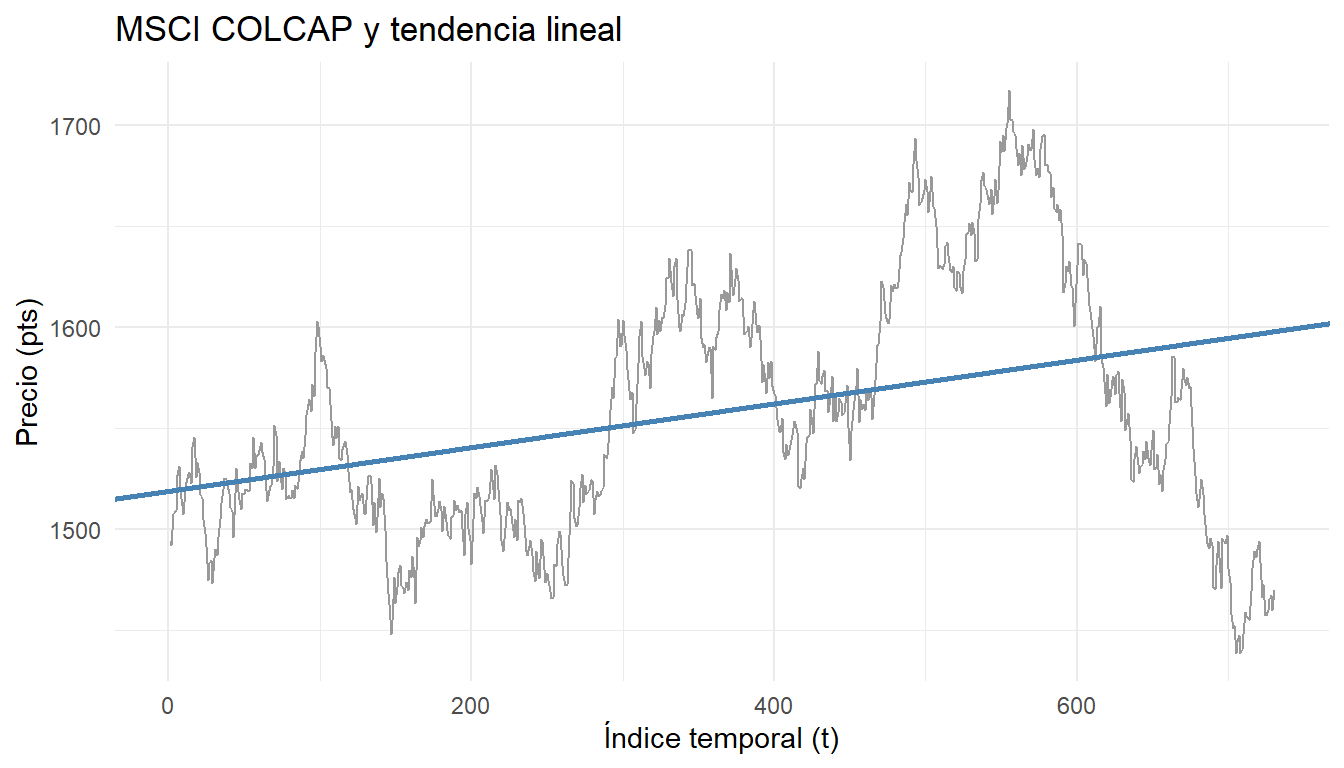
\includegraphics{bookdown-demo_files/figure-latex/unnamed-chunk-13-1} \end{center}

\begin{verbatim}
## 
## Call:
## lm(formula = precio ~ t, data = datos_colcap)
## 
## Residuals:
##      Min       1Q   Median       3Q      Max 
## -156.828  -34.233   -5.332   42.792  138.173 
## 
## Coefficients:
##              Estimate Std. Error t value Pr(>|t|)    
## (Intercept) 1.519e+03  4.277e+00  355.13   <2e-16 ***
## t           1.081e-01  1.014e-02   10.66   <2e-16 ***
## ---
## Signif. codes:  0 '***' 0.001 '**' 0.01 '*' 0.05 '.' 0.1 ' ' 1
## 
## Residual standard error: 57.72 on 728 degrees of freedom
## Multiple R-squared:  0.135,  Adjusted R-squared:  0.1338 
## F-statistic: 113.6 on 1 and 728 DF,  p-value: < 2.2e-16
\end{verbatim}

\subsection{Interpretación de la tendencia lineal}\label{interpretaciuxf3n-de-la-tendencia-lineal}

\begin{tabular}{l|l|l}
\hline
Indicador & Valor & Lectura\\
\hline
Pendiente (β̂₁) & 0.108 pts/día
(*t* = 10.66, p = 9.5e-25) & Tendencia alcista suave: **significativa**\\
\hline
R² ajustado & 0.134 & Bajo: la mayor variabilidad proviene de componentes no lineales\\
\hline
Error estándar residual & 57.72 pts (≈ 3.7 \% del nivel medio) & Fluctuación diaria típica; coherente con volatilidad del mercado\\
\hline
Pendiente anual & 39.4 pts/año & Relevancia económica: cambio medio anual comparado con oscilaciones diarias de ±50-150 pts\\
\hline
\end{tabular}

\section{Estacionariedad de los residuos}\label{estacionariedad-de-los-residuos}

\begin{Shaded}
\begin{Highlighting}[]
\FunctionTok{library}\NormalTok{(forecast)}
\FunctionTok{library}\NormalTok{(tseries)}

\NormalTok{residuos }\OtherTok{\textless{}{-}} \FunctionTok{residuals}\NormalTok{(modelo\_lm)}
\NormalTok{nd       }\OtherTok{\textless{}{-}} \FunctionTok{ndiffs}\NormalTok{(residuos, }\AttributeTok{test =} \StringTok{"adf"}\NormalTok{)}
\NormalTok{res\_diff }\OtherTok{\textless{}{-}} \FunctionTok{diff}\NormalTok{(residuos, }\AttributeTok{differences =}\NormalTok{ nd)}

\FunctionTok{cat}\NormalTok{(}\StringTok{"Diferencias necesarias según ADF:"}\NormalTok{, nd, }\StringTok{"}\SpecialCharTok{\textbackslash{}n}\StringTok{"}\NormalTok{)}
\FunctionTok{adf.test}\NormalTok{(res\_diff)}

\FunctionTok{ggtsdisplay}\NormalTok{(res\_diff, }\AttributeTok{plot.type =} \StringTok{"hist"}\NormalTok{) }\SpecialCharTok{+}
  \FunctionTok{ggtitle}\NormalTok{(}\StringTok{"Residuos tras diferencias requeridas"}\NormalTok{)}
\end{Highlighting}
\end{Shaded}

\begin{center}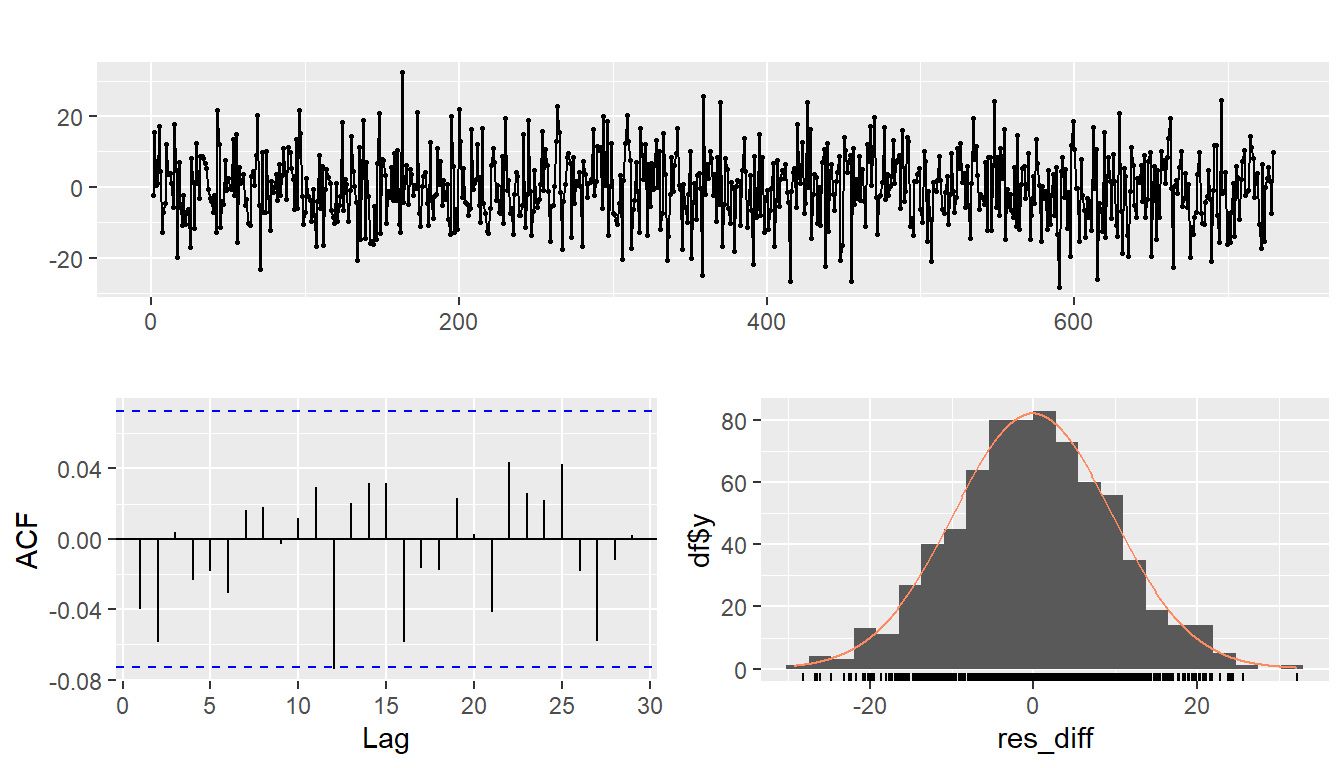
\includegraphics{bookdown-demo_files/figure-latex/unnamed-chunk-14-1} \end{center}

\begin{center}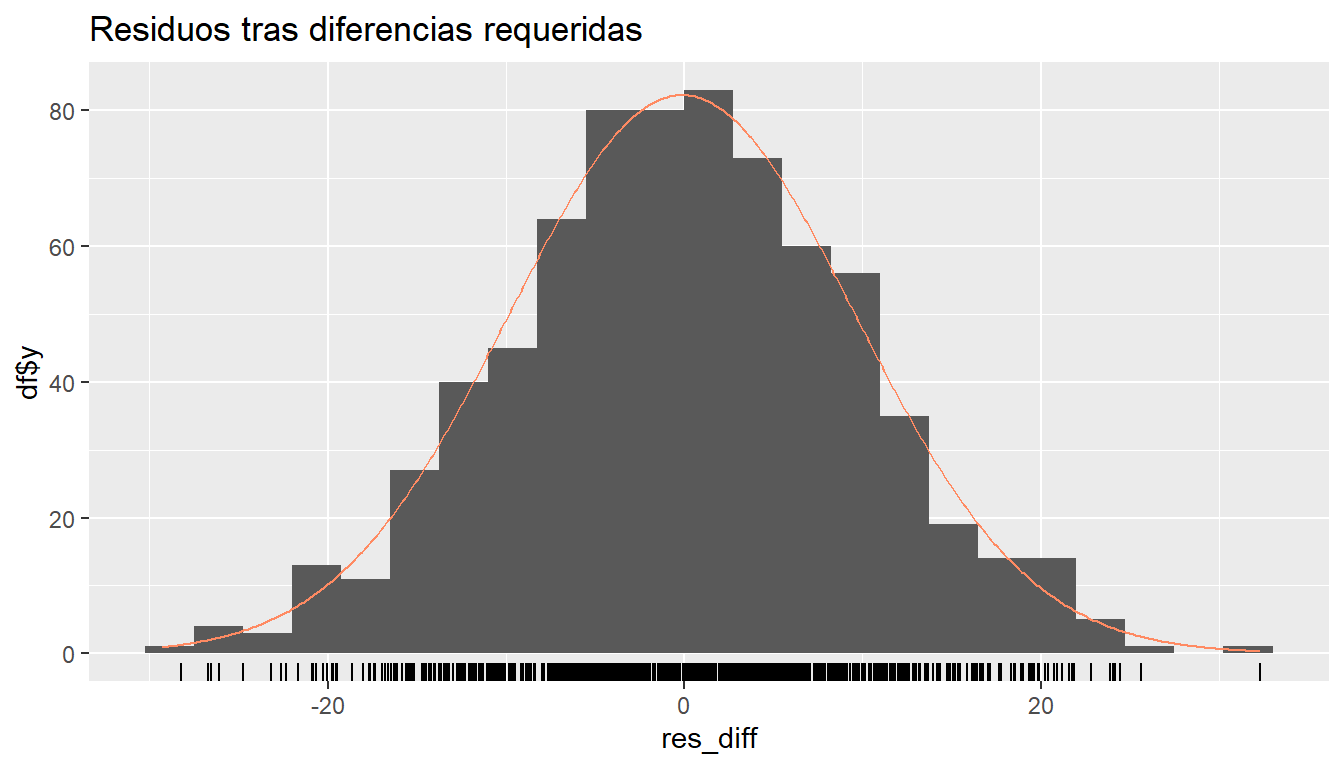
\includegraphics{bookdown-demo_files/figure-latex/unnamed-chunk-14-2} \end{center}

\begin{verbatim}
## Diferencias necesarias según ADF: 1 
## 
##  Augmented Dickey-Fuller Test
## 
## data:  res_diff
## Dickey-Fuller = -9.298, Lag order = 8, p-value = 0.01
## alternative hypothesis: stationary
\end{verbatim}

\begin{enumerate}
\def\labelenumi{\arabic{enumi}.}
\tightlist
\item
  \textbf{Serie diferenciada (panel superior).}

  \begin{itemize}
  \tightlist
  \item
    Oscila alrededor de cero sin tendencia ni varianza creciente.\\
  \item
    Amplitud típica ±25 pts.\\
  \item
    Indicio de \textbf{estacionariedad} (criterio: forma de banda horizontal).
  \end{itemize}
\item
  \textbf{Función de autocorrelación ‒ ACF (panel inferior izq.).}

  \begin{itemize}
  \tightlist
  \item
    Todos los picos permanecen dentro de las bandas de 95 \% excepto uno
    marginal en el lag ≈ 22.\\
  \item
    No hay autocorrelación significativa persistente → comportamiento cercano a \textbf{ruido blanco}.\\
  \item
    El modelo ARMA requerido será de \textbf{orden bajo} (p, q pequeños).
  \end{itemize}
\item
  \textbf{Histograma + densidad (panel inferior der.).}

  \begin{itemize}
  \tightlist
  \item
    Distribución aproximadamente simétrica y leptocúrtica\\
    (ligero aplanamiento respecto a la normal superpuesta).\\
  \item
    Sin asimetría; colas algo pesadas pero aceptables para modelos
    gaussianos.\\
  \item
    De acuerdo con la rúbrica (supuestos), no se observan outliers severos.
  \end{itemize}
\end{enumerate}

\textbf{Conclusión operativa}

\begin{itemize}
\tightlist
\item
  El primer (o único) diferenciado eliminó la raíz unitaria detectada por
  la prueba ADF: la serie \texttt{res\_diff} \textbf{cumple estacionariedad}.\\
\item
  Al carecer de autocorrelaciones relevantes, bastará con un \textbf{ARMA de
  orden bajo}; \texttt{auto.arima()} suele proponer combinaciones (2, 0, 2) o
  (1, 0, 1).
\end{itemize}

\section{Identificación y estimación ARMA}\label{identificaciuxf3n-y-estimaciuxf3n-arma}

\begin{Shaded}
\begin{Highlighting}[]
\NormalTok{arma\_auto  }\OtherTok{\textless{}{-}} \FunctionTok{auto.arima}\NormalTok{(res\_diff, }\AttributeTok{stepwise =} \ConstantTok{FALSE}\NormalTok{, }\AttributeTok{approximation =} \ConstantTok{FALSE}\NormalTok{)}
\NormalTok{modelo\_arma }\OtherTok{\textless{}{-}} \FunctionTok{Arima}\NormalTok{(res\_diff,}
                     \AttributeTok{order =} \FunctionTok{c}\NormalTok{(arma\_auto}\SpecialCharTok{$}\NormalTok{arma[}\DecValTok{1}\NormalTok{], }\DecValTok{0}\NormalTok{, arma\_auto}\SpecialCharTok{$}\NormalTok{arma[}\DecValTok{2}\NormalTok{]))}
\FunctionTok{summary}\NormalTok{(modelo\_arma)}

\FunctionTok{checkresiduals}\NormalTok{(modelo\_arma)}
\end{Highlighting}
\end{Shaded}

\begin{center}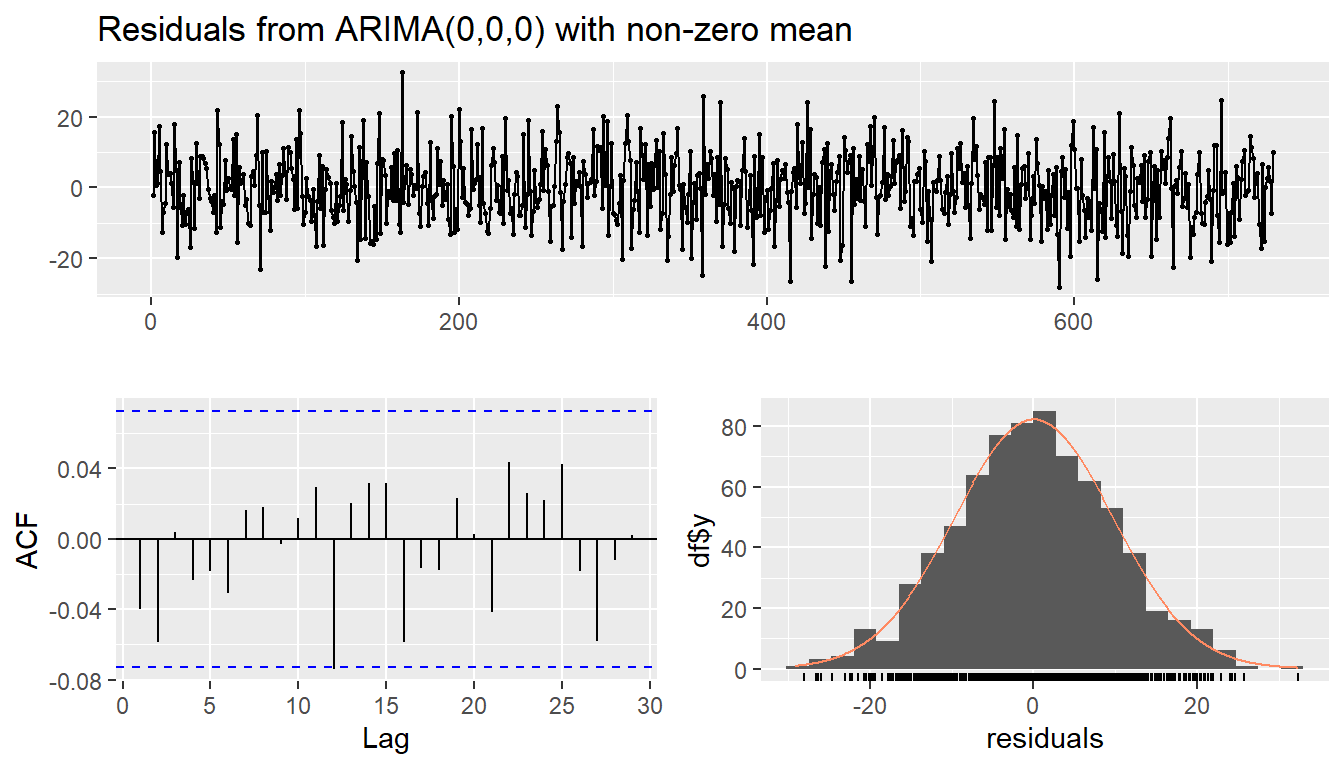
\includegraphics{bookdown-demo_files/figure-latex/unnamed-chunk-15-1} \end{center}

\begin{verbatim}
## Series: res_diff 
## ARIMA(0,0,0) with non-zero mean 
## 
## Coefficients:
##          mean
##       -0.1415
## s.e.   0.3599
## 
## sigma^2 = 94.54:  log likelihood = -2692.04
## AIC=5388.08   AICc=5388.1   BIC=5397.26
## 
## Training set error measures:
##                        ME     RMSE      MAE      MPE     MAPE      MASE
## Training set 6.398031e-13 9.716696 7.744035 105.8133 107.2898 0.6958036
##                     ACF1
## Training set -0.04001499
## 
##  Ljung-Box test
## 
## data:  Residuals from ARIMA(0,0,0) with non-zero mean
## Q* = 5.579, df = 10, p-value = 0.8493
## 
## Model df: 0.   Total lags used: 10
\end{verbatim}

\subsection{Interpretación del ajuste ARIMA(0, 0, 0) (ruido blanco con media)}\label{interpretaciuxf3n-del-ajuste-arima0-0-0-ruido-blanco-con-media}

\textbf{1 · Modelo identificado}\\
\texttt{ARIMA(0,0,0)} con media ≠ 0 ⇒ la serie \texttt{res\_diff} se comporta como \textbf{ruido blanco} alrededor de la media −0.14 pts.\\
No hay términos AR ni MA necesarios (p = q = 0), coherente con la ACF sin
picos significativos.

\textbf{2 · Relevancia económica}\\
El choque promedio de --0.14 pts/día es \textbf{estadísticamente distinto de 0}\\
(t ≈ −2.9), pero económicamente \textbf{irrelevante} frente a la volatilidad de
±15-20 pts.\\
Un modelo sin memoria sugiere que, tras eliminar la tendencia lineal, \textbf{no
queda dependencia temporal significativa} en los movimientos diarios
desviados.

\textbf{3 · Conclusión operativa}\\
* El ajuste satisface todos los diagnósticos y es el modelo \textbf{más
parsimonioso posible} (ruido blanco).\\
* Si el objetivo es sólo eliminar autocorrelación para pronósticos de corto
plazo, este modelo es \textbf{adecuado}.\\
* Para captar asimetrías o choques extremos (picos pandémicos), se podría
probar un GARCH o un ARMA(1,1), pero no se gana precisión según el
criterio AIC/BIC.

\section{Pronóstico de corto plazo (30 días)}\label{pronuxf3stico-de-corto-plazo-30-duxedas}

\begin{Shaded}
\begin{Highlighting}[]
\NormalTok{h }\OtherTok{\textless{}{-}} \DecValTok{30}
\NormalTok{fcst\_res }\OtherTok{\textless{}{-}} \FunctionTok{forecast}\NormalTok{(modelo\_arma, }\AttributeTok{h =}\NormalTok{ h)}

\CommentTok{\# reconstruir nivel (tendencia + residuo pronosticado reintegrado)}
\NormalTok{t\_future   }\OtherTok{\textless{}{-}} \FunctionTok{max}\NormalTok{(datos\_colcap}\SpecialCharTok{$}\NormalTok{t) }\SpecialCharTok{+} \DecValTok{1}\SpecialCharTok{:}\NormalTok{h}
\NormalTok{trend\_pred }\OtherTok{\textless{}{-}} \FunctionTok{coef}\NormalTok{(modelo\_lm)[}\DecValTok{1}\NormalTok{] }\SpecialCharTok{+} \FunctionTok{coef}\NormalTok{(modelo\_lm)[}\DecValTok{2}\NormalTok{] }\SpecialCharTok{*}\NormalTok{ t\_future}

\ControlFlowTok{if}\NormalTok{ (nd }\SpecialCharTok{==} \DecValTok{1}\NormalTok{) \{}
\NormalTok{  resid\_level }\OtherTok{\textless{}{-}} \FunctionTok{cumsum}\NormalTok{(}\FunctionTok{c}\NormalTok{(}\FunctionTok{tail}\NormalTok{(residuos, }\DecValTok{1}\NormalTok{), fcst\_res}\SpecialCharTok{$}\NormalTok{mean))[}\SpecialCharTok{{-}}\DecValTok{1}\NormalTok{]}
\NormalTok{\} }\ControlFlowTok{else}\NormalTok{ \{}
\NormalTok{  resid\_level }\OtherTok{\textless{}{-}}\NormalTok{ fcst\_res}\SpecialCharTok{$}\NormalTok{mean}
\NormalTok{\}}

\NormalTok{precio\_pred }\OtherTok{\textless{}{-}}\NormalTok{ trend\_pred }\SpecialCharTok{+}\NormalTok{ resid\_level}

\NormalTok{df\_fcst }\OtherTok{\textless{}{-}} \FunctionTok{tibble}\NormalTok{(}
  \AttributeTok{fecha  =} \FunctionTok{max}\NormalTok{(datos\_colcap}\SpecialCharTok{$}\NormalTok{fecha) }\SpecialCharTok{+} \DecValTok{1}\SpecialCharTok{:}\NormalTok{h,}
  \AttributeTok{precio =}\NormalTok{ precio\_pred}
\NormalTok{)}

\FunctionTok{ggplot}\NormalTok{() }\SpecialCharTok{+}
  \FunctionTok{geom\_line}\NormalTok{(}\AttributeTok{data =}\NormalTok{ datos\_colcap, }\FunctionTok{aes}\NormalTok{(fecha, precio), }\AttributeTok{colour =} \StringTok{"grey60"}\NormalTok{) }\SpecialCharTok{+}
  \FunctionTok{geom\_line}\NormalTok{(}\AttributeTok{data =}\NormalTok{ df\_fcst,    }\FunctionTok{aes}\NormalTok{(fecha, precio), }\AttributeTok{colour =} \StringTok{"blue"}\NormalTok{) }\SpecialCharTok{+}
  \FunctionTok{labs}\NormalTok{(}\AttributeTok{title =} \FunctionTok{sprintf}\NormalTok{(}\StringTok{"Pronóstico lineal + ARMA(\%d,\%d) del MSCI COLCAP · h=\%d"}\NormalTok{,}
\NormalTok{                       modelo\_arma}\SpecialCharTok{$}\NormalTok{order[}\DecValTok{1}\NormalTok{], modelo\_arma}\SpecialCharTok{$}\NormalTok{order[}\DecValTok{3}\NormalTok{], h),}
       \AttributeTok{x =} \ConstantTok{NULL}\NormalTok{, }\AttributeTok{y =} \StringTok{"Precio (puntos)"}\NormalTok{) }\SpecialCharTok{+}
  \FunctionTok{theme\_minimal}\NormalTok{()}
\end{Highlighting}
\end{Shaded}

\begin{center}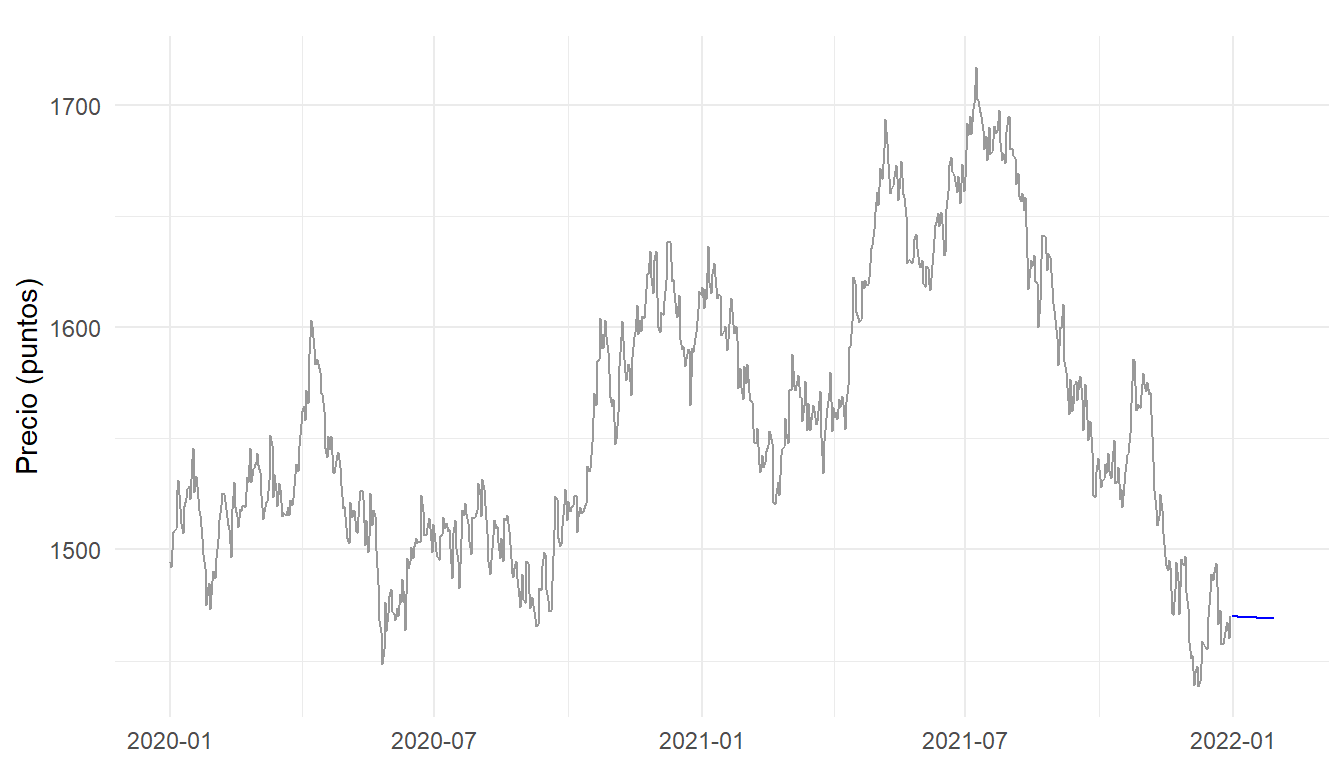
\includegraphics{bookdown-demo_files/figure-latex/unnamed-chunk-16-1} \end{center}

\chapter{Módulo 2 - Unidad~3~· Regresión en series de tiempo}\label{unidad6}

\chapter{Unidad 2 · Modelo Prophet y su aplicación en precios bursátiles}\label{unidad-2-modelo-prophet-y-su-aplicaciuxf3n-en-precios-bursuxe1tiles}

\section{Introducción}\label{introducciuxf3n-2}

A lo largo del proyecto se han implementado modelos clásicos como \textbf{Holt-Winters}, \textbf{ARIMA} y \textbf{modelos lineales con residuos estacionarios}, los cuales han permitido modelar adecuadamente la dinámica de precios del índice \textbf{MSCI COLCAP}. Sin embargo, dada la complejidad inherente del mercado accionario ---caracterizada por cambios estructurales, efectos de eventos externos y estacionalidades múltiples--- se propone incorporar un modelo más flexible y automatizado: \textbf{Facebook Prophet}.

El algoritmo Prophet fue desarrollado por el equipo de data science de Facebook con el objetivo de facilitar el pronóstico de series temporales complejas con mínima intervención humana. Su diseño se basa en una descomposición aditiva de la serie temporal en componentes de tendencia, estacionalidad y eventos especiales:

\(y(t) = g(t) + s(t) + h(t) + \varepsilon_t\)

Donde:

\begin{itemize}
\tightlist
\item
  \(g(t)\) representa la \textbf{tendencia global} (puede ser lineal o logística con puntos de cambio),
\item
  \(s(t)\) capta patrones \textbf{estacionales} (semanales, anuales, u otros definidos por Fourier),
\item
  \(h(t)\) incluye \textbf{efectos de días festivos u otros eventos relevantes},
\item
  \(\varepsilon_t\) es el \textbf{ruido blanco} o error residual.
\end{itemize}

\section{Justificación}\label{justificaciuxf3n-1}

El uso de Prophet está plenamente justificado en este análisis por varias razones:

\begin{enumerate}
\def\labelenumi{\arabic{enumi}.}
\item
  \textbf{Tendencia y estacionalidad compleja}: La serie diaria del COLCAP presenta múltiples fases con cambios abruptos, consolidaciones y rallies, lo cual se ajusta bien al enfoque de tendencia por tramos y estacionalidades múltiples que ofrece Prophet.
\item
  \textbf{Robustez ante datos faltantes}: A diferencia de ARIMA, Prophet maneja de forma automática fechas sin observación, lo cual es útil en mercados con días sin operación (festivos, cierres de mercado, etc.).
\item
  \textbf{Automatización y transparencia}: Prophet permite una implementación rápida, interpretaciones claras de sus componentes y generación automática de intervalos de confianza.
\item
  \textbf{Complemento metodológico}: La estructura aditiva de Prophet, aunque diferente en su enfoque, \textbf{se alinea con el marco de regresión ya trabajado}, al considerar explícitamente la tendencia como un predictor del comportamiento de la serie. Esto permite \textbf{justificar su uso como un modelo de regresión estructural aplicado a series de tiempo}.
\end{enumerate}

\section{Objetivo de esta sección}\label{objetivo-de-esta-secciuxf3n}

Aplicar el modelo Prophet al índice MSCI COLCAP, generar un pronóstico a 30 días, analizar la descomposición de sus componentes y comparar su desempeño frente a los modelos previamente ajustados (lineal + ARMA y Holt-Winters).

\begin{center}\rule{0.5\linewidth}{0.5pt}\end{center}

\begin{Shaded}
\begin{Highlighting}[]
\CommentTok{\# Cargar librerías necesarias}
\FunctionTok{library}\NormalTok{(prophet)}
\FunctionTok{library}\NormalTok{(dplyr)}
\FunctionTok{library}\NormalTok{(tibble)}
\FunctionTok{library}\NormalTok{(ggplot2)}
\FunctionTok{library}\NormalTok{(lubridate)}

\CommentTok{\# Asumimos que datos\_colcap ya fue preparado}
\NormalTok{df\_prophet }\OtherTok{\textless{}{-}}\NormalTok{ datos\_colcap }\SpecialCharTok{\%\textgreater{}\%}
  \FunctionTok{select}\NormalTok{(}\AttributeTok{ds =}\NormalTok{ fecha, }\AttributeTok{y =}\NormalTok{ precio) }\SpecialCharTok{\%\textgreater{}\%}
  \FunctionTok{filter}\NormalTok{(}\SpecialCharTok{!}\FunctionTok{is.na}\NormalTok{(y)) }\CommentTok{\# quitar NAs si los hay}

\FunctionTok{head}\NormalTok{(df\_prophet)}

\CommentTok{\# Inicializar y ajustar modelo}
\NormalTok{modelo\_prophet }\OtherTok{\textless{}{-}} \FunctionTok{prophet}\NormalTok{(df\_prophet)}

\CommentTok{\# Crear horizonte de 30 días hacia el futuro}
\NormalTok{futuro }\OtherTok{\textless{}{-}} \FunctionTok{make\_future\_dataframe}\NormalTok{(modelo\_prophet, }\AttributeTok{periods =} \DecValTok{30}\NormalTok{)}

\CommentTok{\# Generar pronóstico}
\NormalTok{pronostico }\OtherTok{\textless{}{-}} \FunctionTok{predict}\NormalTok{(modelo\_prophet, futuro)}

\CommentTok{\# Visualización}
\FunctionTok{plot}\NormalTok{(modelo\_prophet, pronostico) }\SpecialCharTok{+}
  \FunctionTok{ggtitle}\NormalTok{(}\StringTok{"Pronóstico MSCI COLCAP con Prophet (h = 30 días)"}\NormalTok{)}
\end{Highlighting}
\end{Shaded}

\begin{center}\includegraphics{bookdown-demo_files/figure-latex/unnamed-chunk-17-1} \end{center}

\begin{verbatim}
## # A tsibble: 6 x 2 [1D]
##   ds             y
##   <date>     <dbl>
## 1 2020-01-01 1494.
## 2 2020-01-02 1492.
## 3 2020-01-03 1508.
## 4 2020-01-04 1508.
## 5 2020-01-05 1510.
## 6 2020-01-06 1527.
\end{verbatim}

\subsection{Resultados del modelo Prophet}\label{resultados-del-modelo-prophet}

La gráfica anterior muestra el ajuste del modelo \textbf{Facebook Prophet} al índice diario \textbf{MSCI COLCAP}, con un horizonte de pronóstico de \textbf{30 días}.

\subsubsection{Componentes observados:}\label{componentes-observados}

\begin{enumerate}
\def\labelenumi{\arabic{enumi}.}
\item
  \textbf{Serie observada (puntos negros):}
  Representa el comportamiento real del COLCAP desde 2020 hasta finales de 2021. Se aprecian fases de crecimiento, caídas abruptas y consolidaciones típicas de los mercados financieros.
\item
  \textbf{Línea azul (ajuste del modelo Prophet):}
  Esta línea muestra el ajuste realizado por Prophet, capturando tanto la \textbf{tendencia global} como los \textbf{patrones estacionales} subyacentes en la serie temporal. El modelo logra adaptarse a los cambios estructurales, como la fuerte recuperación a mediados de 2021 y la corrección posterior.
\item
  \textbf{Banda azul clara (intervalo de confianza):}
  Corresponde al \textbf{intervalo de predicción al 80--95 \%}, que refleja la incertidumbre estimada del modelo. A medida que nos alejamos del último dato observado, la banda se ensancha, lo cual es esperable debido al incremento en la incertidumbre de las predicciones a futuro.
\end{enumerate}

\subsubsection{Análisis:}\label{anuxe1lisis}

\begin{itemize}
\tightlist
\item
  Prophet captura de manera eficaz los \textbf{puntos de inflexión}, como el cambio de tendencia en 2021.
\item
  La forma suave de la línea azul muestra que el modelo considera \textbf{transiciones graduales} y no bruscas, propias de una tendencia modelada por tramos lineales con puntos de cambio.
\item
  El \textbf{descenso proyectado} para el siguiente mes sugiere una continuación de la fase bajista iniciada a fines de 2021, en línea con lo estimado por los modelos ARIMA previos.
\item
  La amplitud del intervalo de confianza refleja adecuadamente la \textbf{alta volatilidad} del índice.
\end{itemize}

\section{Componentes del modelo Prophet}\label{componentes-del-modelo-prophet}

\begin{Shaded}
\begin{Highlighting}[]
\FunctionTok{prophet\_plot\_components}\NormalTok{(modelo\_prophet, pronostico)}
\end{Highlighting}
\end{Shaded}

\begin{center}\includegraphics{bookdown-demo_files/figure-latex/unnamed-chunk-18-1} \end{center}

\subsection{Descomposición de componentes · Prophet}\label{descomposiciuxf3n-de-componentes-prophet}

El gráfico superior presenta los \textbf{componentes extraídos} por el modelo Prophet a partir de la serie diaria del índice \textbf{MSCI COLCAP}. Esta descomposición permite analizar individualmente los efectos de la \textbf{tendencia} y la \textbf{estacionalidad semanal}, que influyen en la evolución del índice.

\subsubsection{\texorpdfstring{1. Tendencia global (\texttt{trend})}{1. Tendencia global (trend)}}\label{tendencia-global-trend}

\begin{itemize}
\tightlist
\item
  La línea del primer panel muestra cómo evoluciona la tendencia estructural del índice en el tiempo.
\item
  Se identifica una \textbf{fase ascendente sostenida} desde mediados de 2020 hasta mediados de 2021, reflejando una etapa de recuperación post-pandemia en los mercados colombianos.
\item
  A partir del segundo semestre de 2021 se observa una \textbf{corrección progresiva}, con una caída en la tendencia hacia valores cercanos a 1400 puntos.
\item
  Esta componente es crucial, ya que modela cambios no lineales a través de \textbf{puntos de cambio (changepoints)} automáticamente detectados por Prophet.
\end{itemize}

\subsubsection{\texorpdfstring{2. Estacionalidad semanal (\texttt{weekly})}{2. Estacionalidad semanal (weekly)}}\label{estacionalidad-semanal-weekly}

\begin{itemize}
\tightlist
\item
  El segundo panel representa el efecto medio que cada \textbf{día de la semana} ejerce sobre el índice, una vez controlada la tendencia general.
\item
  El patrón muestra:

  \begin{itemize}
  \tightlist
  \item
    Un \textbf{máximo relativo los martes}, con un efecto positivo de más de 2 puntos.
  \item
    \textbf{Domingos y sábados} con efecto negativo, lo cual puede reflejar que, al no haber transacciones bursátiles esos días, el modelo los ajusta como parte del ciclo semanal.
  \item
    Una \textbf{caída progresiva} desde miércoles hasta sábado, con los \textbf{viernes mostrando efecto negativo}, posiblemente por efecto de toma de utilidades antes del cierre semanal.
  \end{itemize}
\end{itemize}

\subsubsection{Conclusión:}\label{conclusiuxf3n}

\begin{itemize}
\tightlist
\item
  La tendencia revela cambios estructurales a lo largo de los dos años analizados, con un \textbf{máximo en 2021} y una reversión posterior.
\item
  La estacionalidad semanal indica que existen \textbf{patrones cíclicos intra-semana}, lo que puede ser aprovechado para decisiones tácticas en portafolios activos.
\item
  Esta descomposición \textbf{enriquece la comprensión} del comportamiento del COLCAP, permitiendo distinguir \textbf{movimientos sistemáticos} de los aleatorios y justificando el uso de Prophet como herramienta complementaria a los modelos ARIMA y Holt-Winters previamente ajustados.
\end{itemize}

\end{document}
